%Title: Fus. evap results for U and Th isotopes
%Author: A. Raggio
%Year: 2020

\documentclass[10pt]{beamer}

%
%Setting file
%

\usepackage[T1]{fontenc}
\usepackage[utf8]{inputenc}

\usepackage[english]{babel}

\usepackage{graphicx}
\graphicspath{{images/}}
\usepackage{float}
\usepackage{tikz}
\usepackage{caption}
\usepackage{subcaption}

\usetheme{default}
\usefonttheme{structurebold}


% ---------------------------------
% color definitions
\usepackage{color}
% \definecolor{LISA_BLUE}{rgb}{0.25,0.33,0.66}
\definecolor{LISA_BLUE}{cmyk}{0.99,0.88,0.29,0.18}

\setbeamercolor{normal text}{fg=LISA_BLUE}
\setbeamercolor{frametitle}{fg=LISA_BLUE}

\newcommand\insertlocation{}  % Empty by default.
\newcommand\location[1]{\renewcommand\insertlocation{#1}}

\newcommand\insertperiod{}  % Empty by default.
\newcommand\period[1]{\renewcommand\insertperiod{#1}}



\setbeamertemplate{itemize items}[circle]
\setbeamercolor{title}{fg=white}



%-----------------------------------------Title page settings-----------------------------------------%
\title{ Decay Spectroscopy\\ Measurement at IGISOL}

\institute{}

\author{}


\date{}
\titlegraphic{% 
\vspace{0.05\textheight}
	\centering
	
\includegraphics[height=3cm]{jyu-keskitetty-kaksikielinen.eps}\\
\vspace{-0.03\textheight}
}
%-----------------------------------------Title page settings-----------------------------------------%


\setbeamertemplate{footline}
{
 \begin{beamercolorbox}{section in head/foot}
 \vskip2pt\hspace{0.095cm} Andrea Raggio \hfill Jyv\"{a}skyl\"{a} - 13 November 2020 \hspace{0.15cm}\phantom{x}\vskip2pt
 \end{beamercolorbox}%
}


\begin{document}
\frame{\titlepage}

\section{Introduction}

\begin{frame}{Introduction}
\begin{columns}
	\begin{column}{0.5\textwidth}
		\begin{overlayarea}{\textwidth}{\textheight}
			\centering
			\vspace{0.2\textheight}		
			\begin{itemize}
				\item<1-> Physics Case
				\item<2-> Experimental Setup
				\item<3-> Preliminary Efficiency Test
			\end{itemize}
		\end{overlayarea}
	\end{column}
	\begin{column}{0.5\textwidth}
		\begin{overlayarea}{\textwidth}{\textheight}
			\centering
			\only<1>{\vspace{0.12\textheight}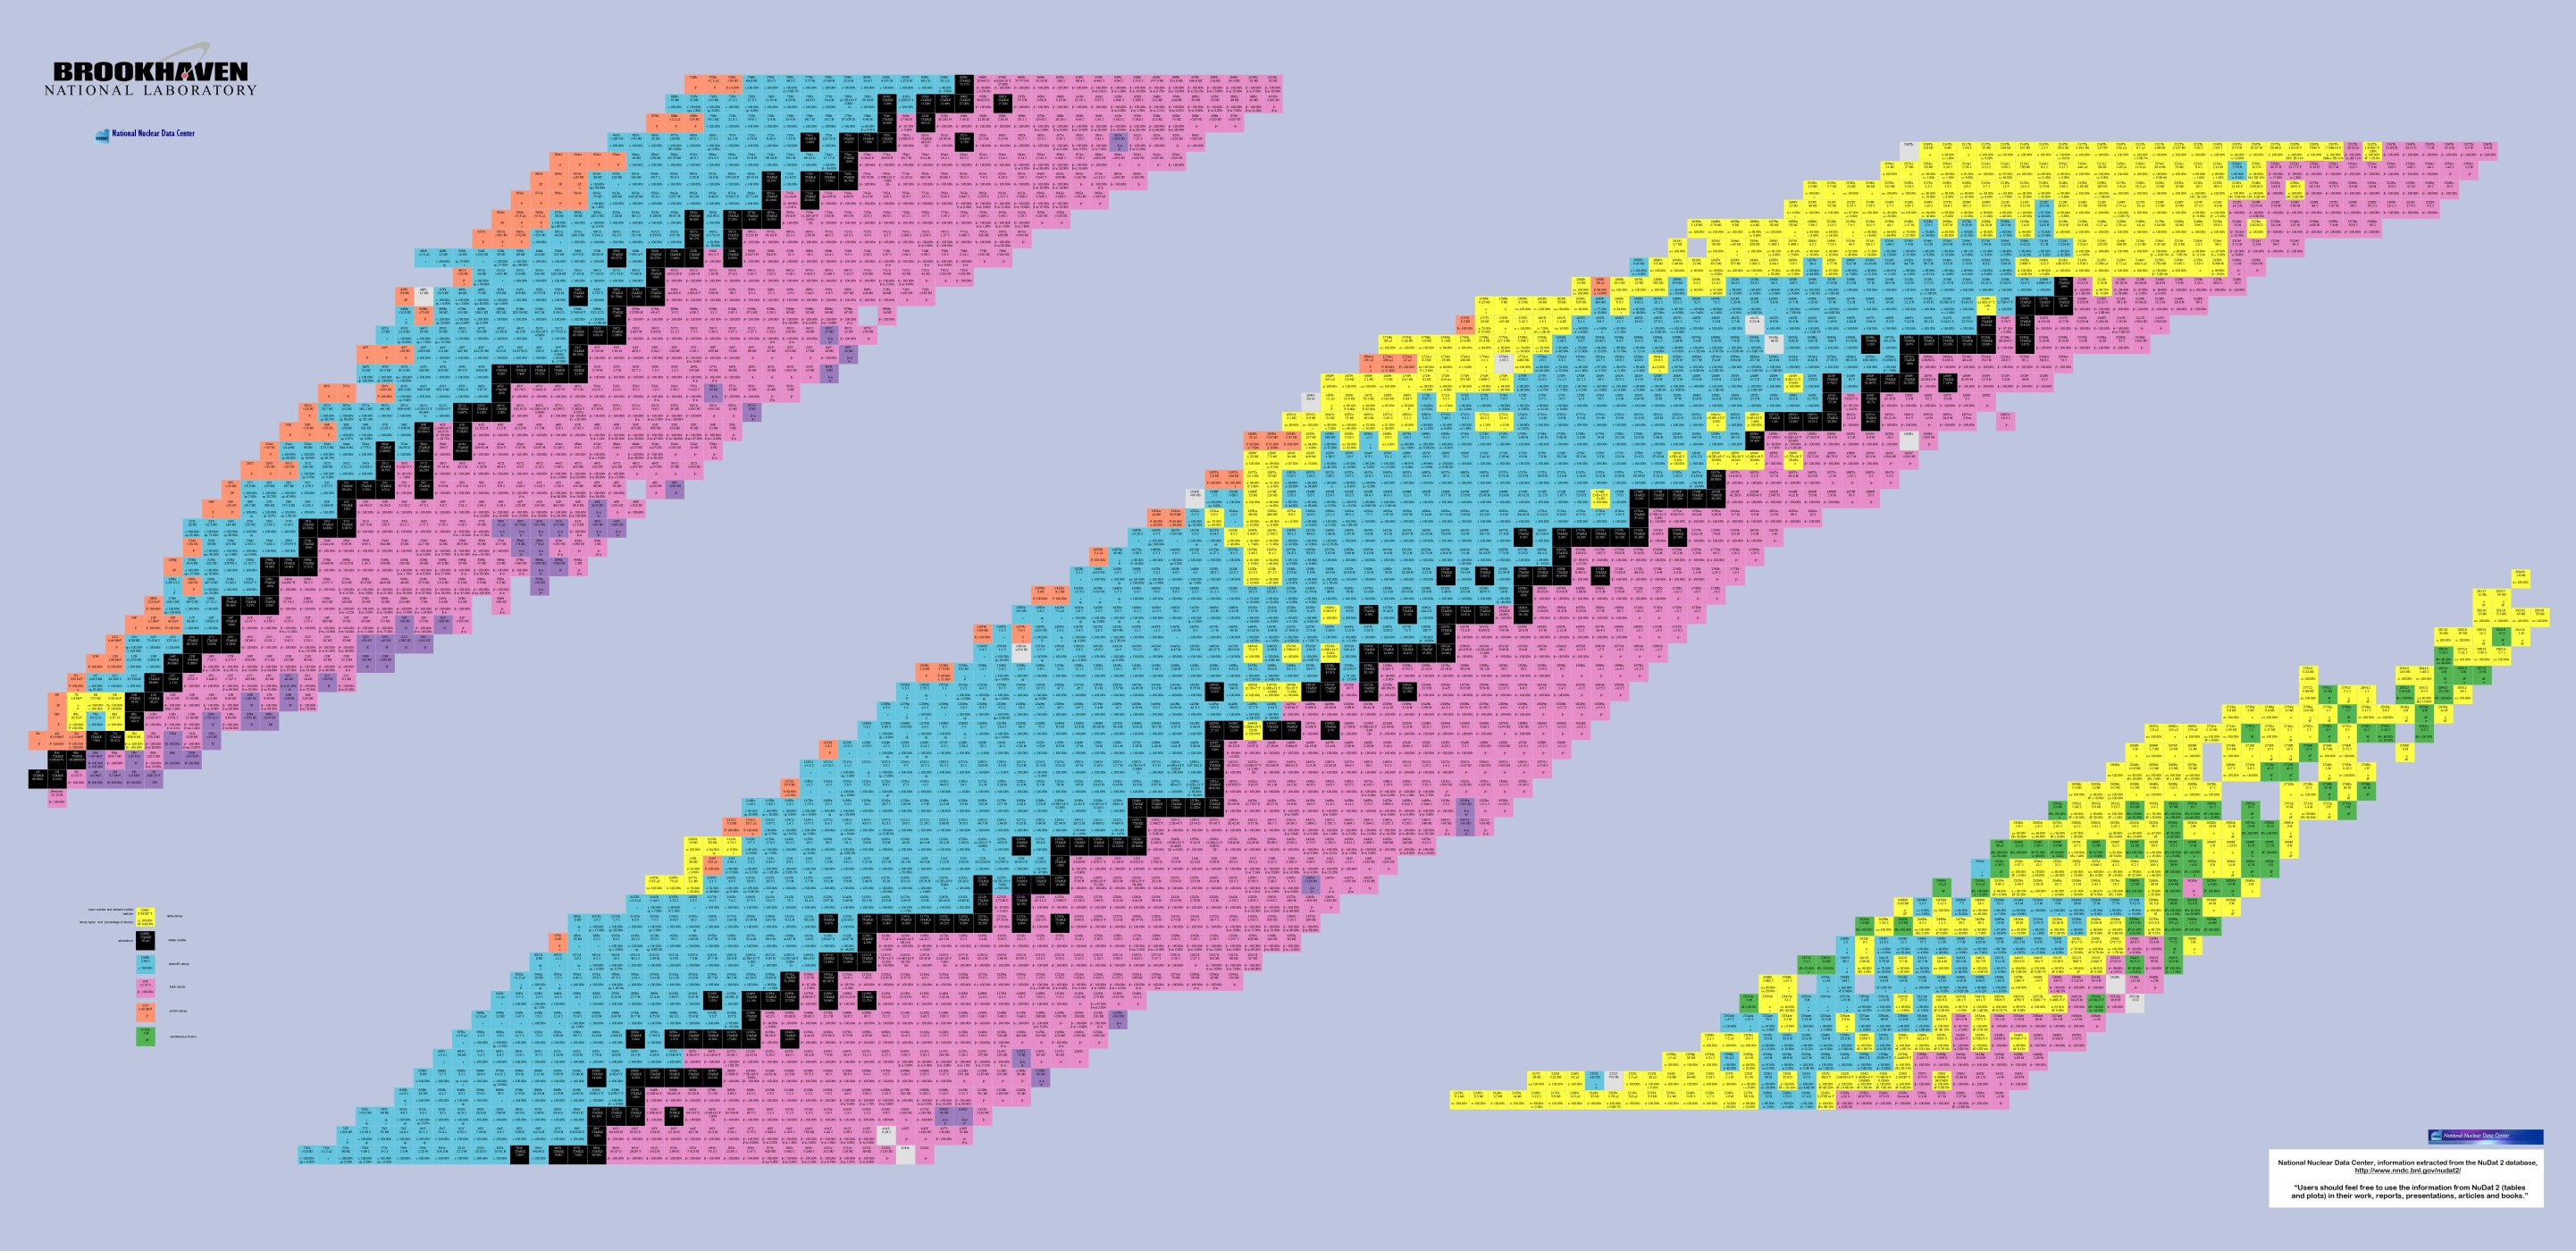
\includegraphics[width=1.\textwidth]{phycase.jpg}\\}
			\only<2>{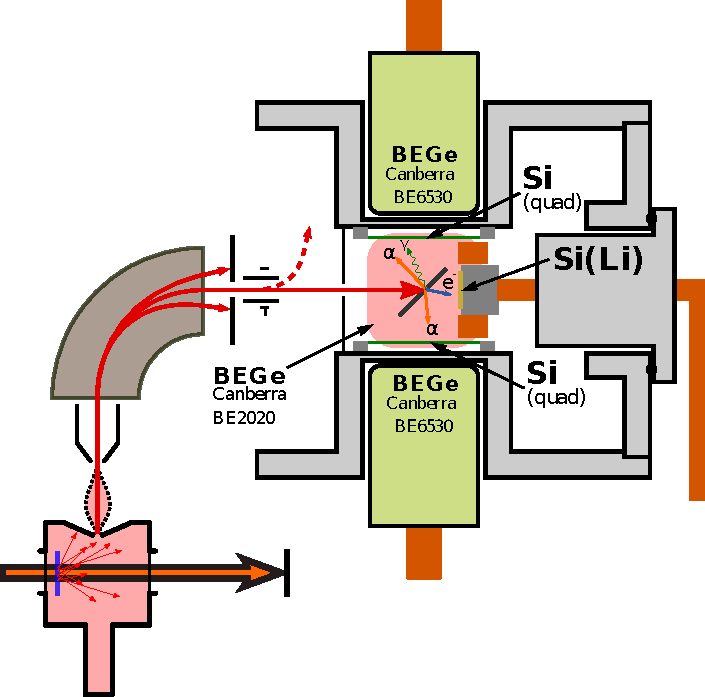
\includegraphics[width=1.\textwidth]{Total_setup.pdf}\\}
			\only<3>{\vspace{0.1\textheight}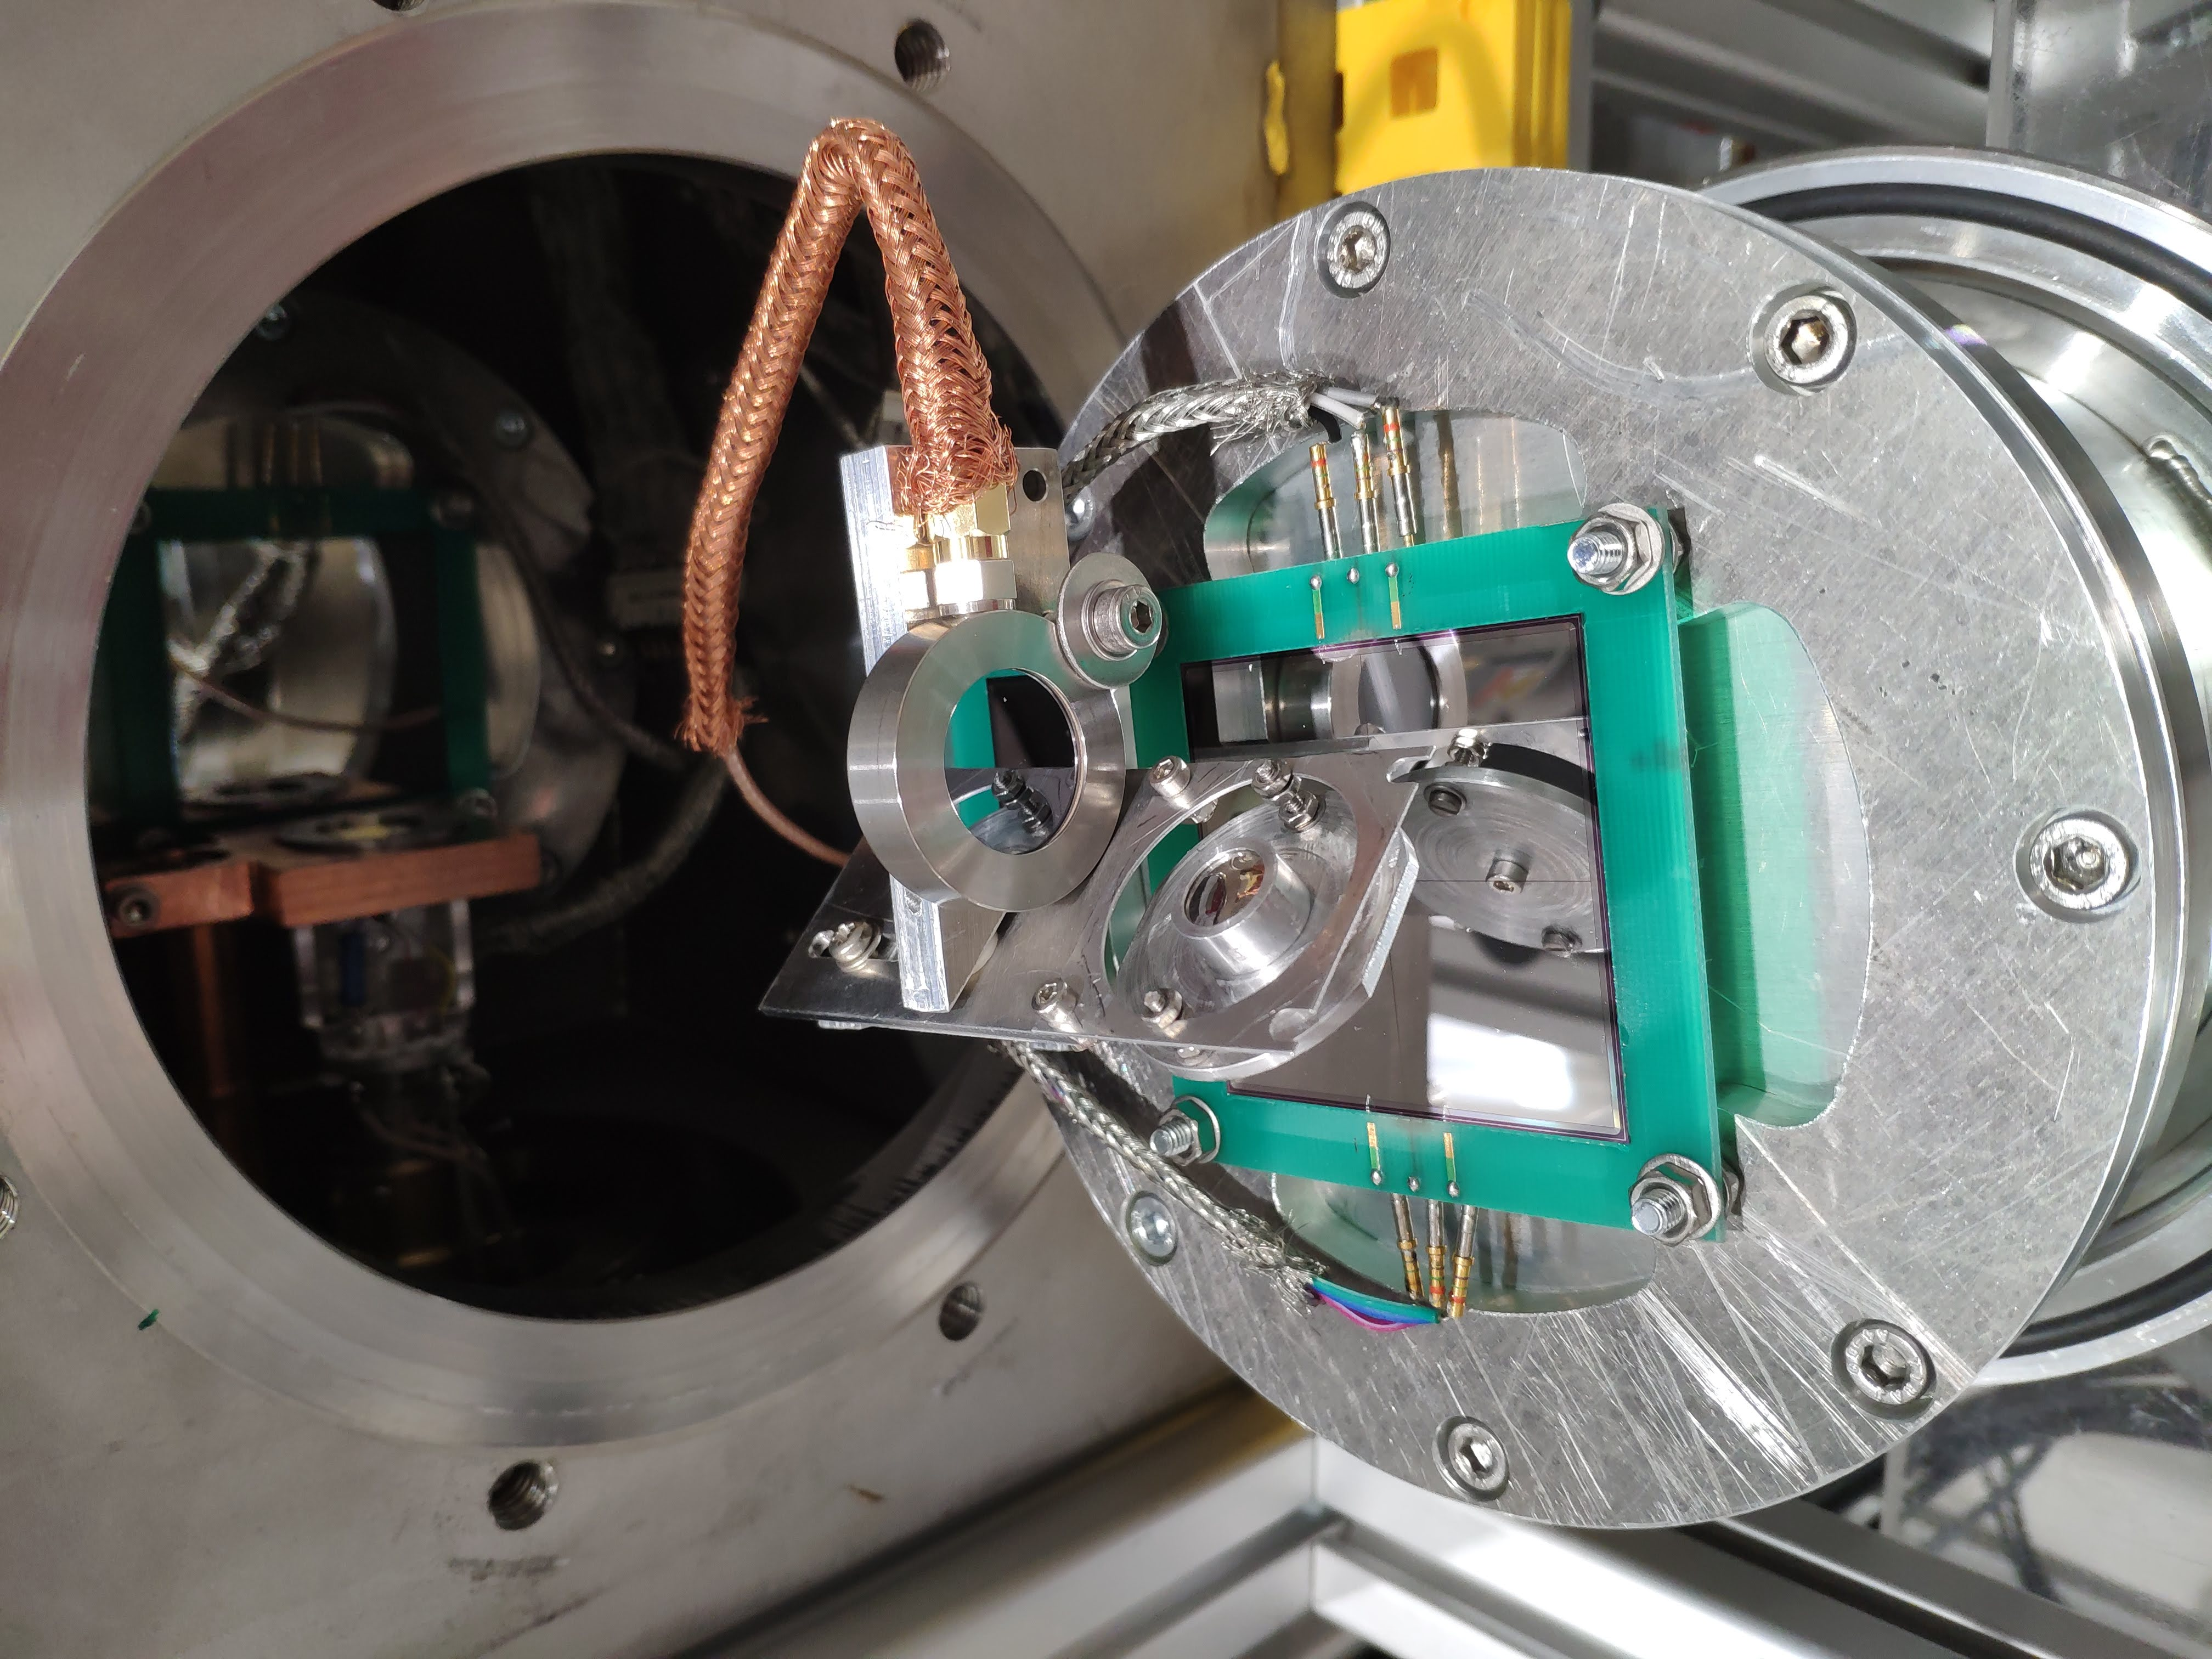
\includegraphics[angle=-90,origin=c,width=0.45\textwidth]{3alpha.jpg}
				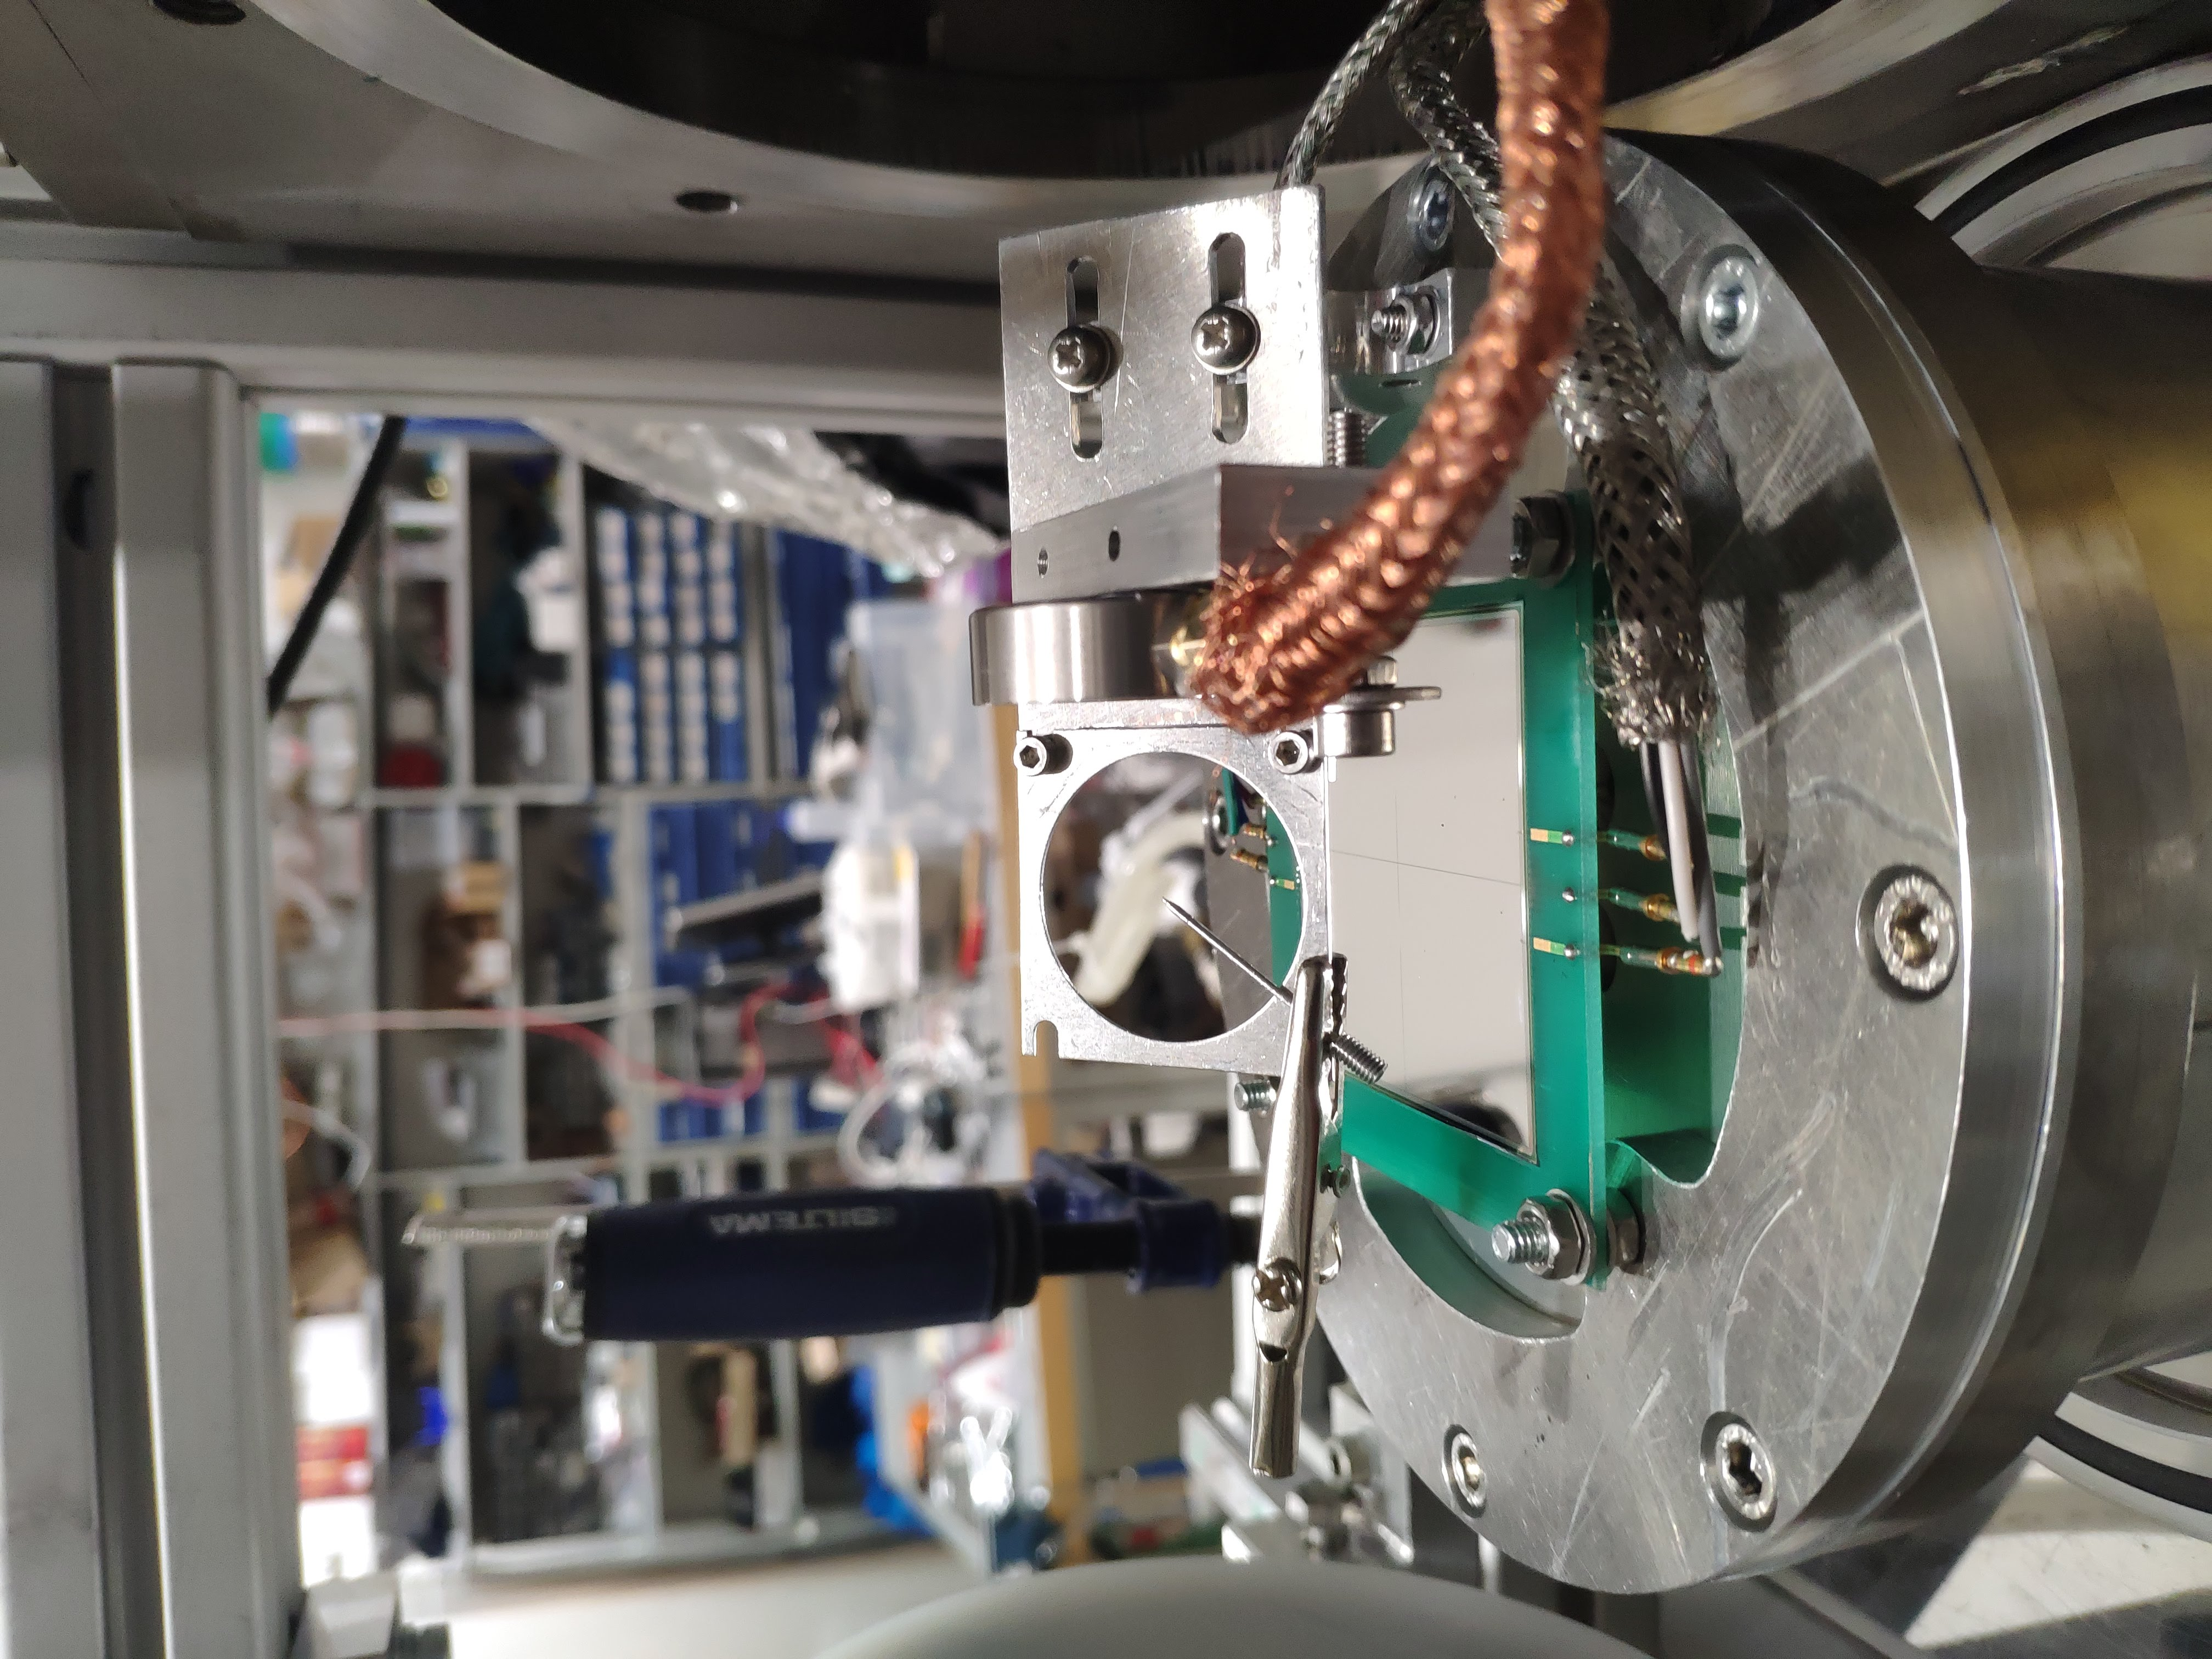
\includegraphics[angle=-90,origin=c,width=0.45\textwidth]{alpharec.jpg}}
		\end{overlayarea}
	\end{column}
\end{columns}
\end{frame}

\section{Physics Case}
\begin{frame}{Motivation}
	\begin{overlayarea}{\textwidth}{\textheight}
		\centering
		%\vspace{-0.05\textheight}
		\only<1>{\includegraphics[width=1.\textwidth]{case_0.png}\\}
		\only<2>{\includegraphics[width=1.\textwidth]{case_1.png}\\}
	\end{overlayarea}
\end{frame}

\begin{frame}{Reaction}
	\begin{overlayarea}{\textwidth}{\textheight}
		\centering
		\vspace{-0.1\textheight}
		\only<1->{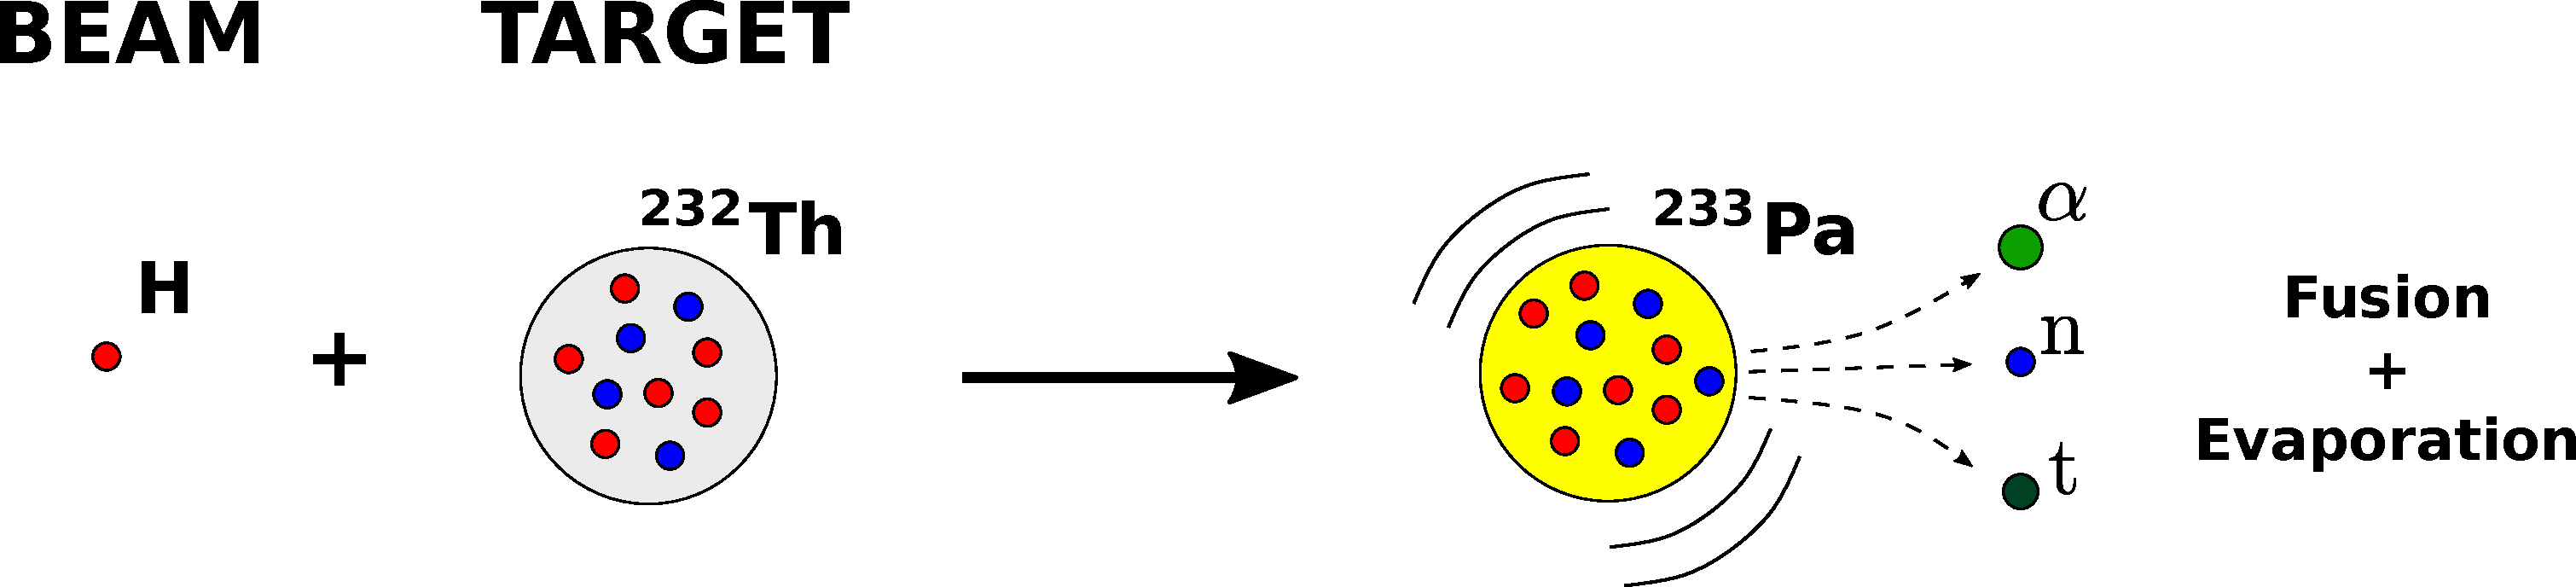
\includegraphics[width=0.8\textwidth]{Reaction.pdf}\\}
		%\vspace{0.1\textheight}
		\begin{itemize}
		\small
			\item<2-> 65~MeV Hydrogen Beam on $^{232}$Th target 
			\item<3->Evaporated residual extracted, selected and implanted on Carbon foil at spectroscopy setup.
		\end{itemize}
		\only<1>{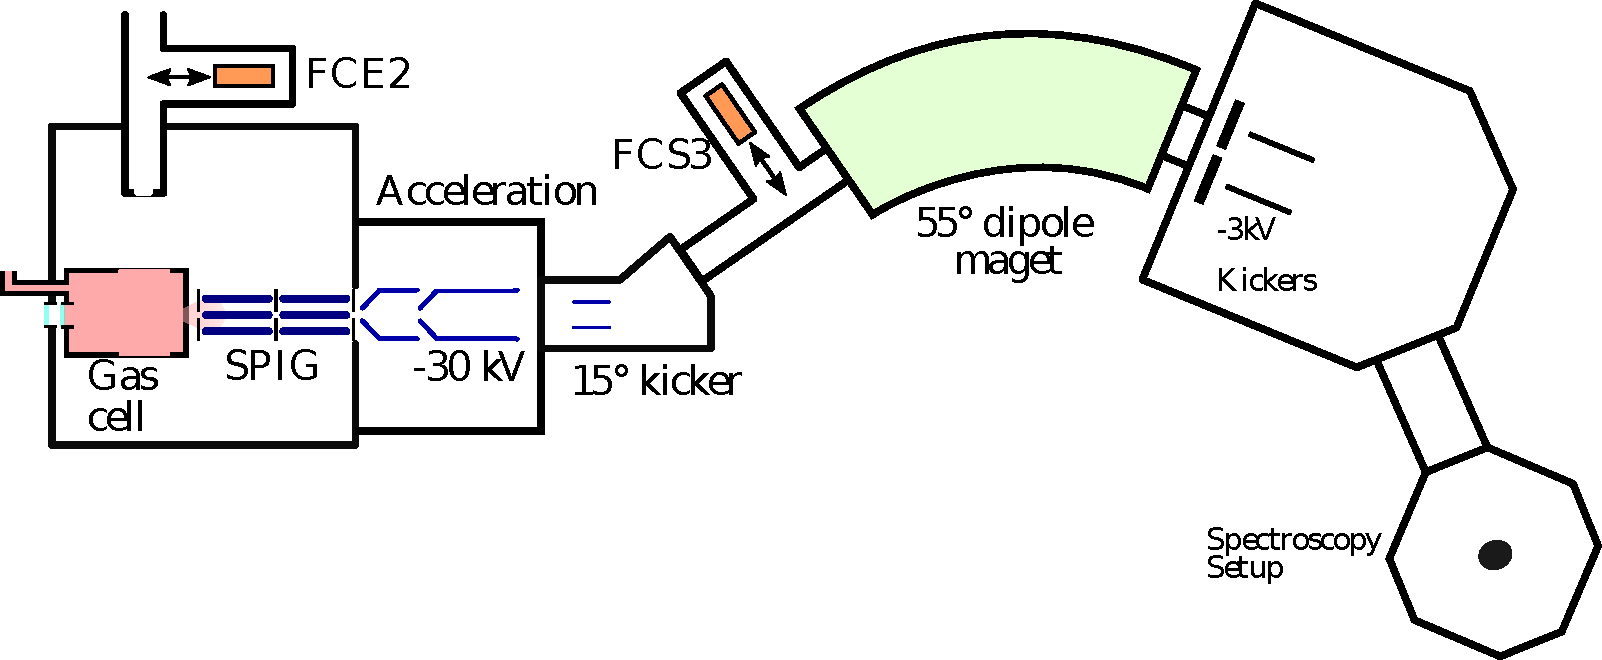
\includegraphics[width=0.8\textwidth]{IGISOL_1}\\}
		\only<2>{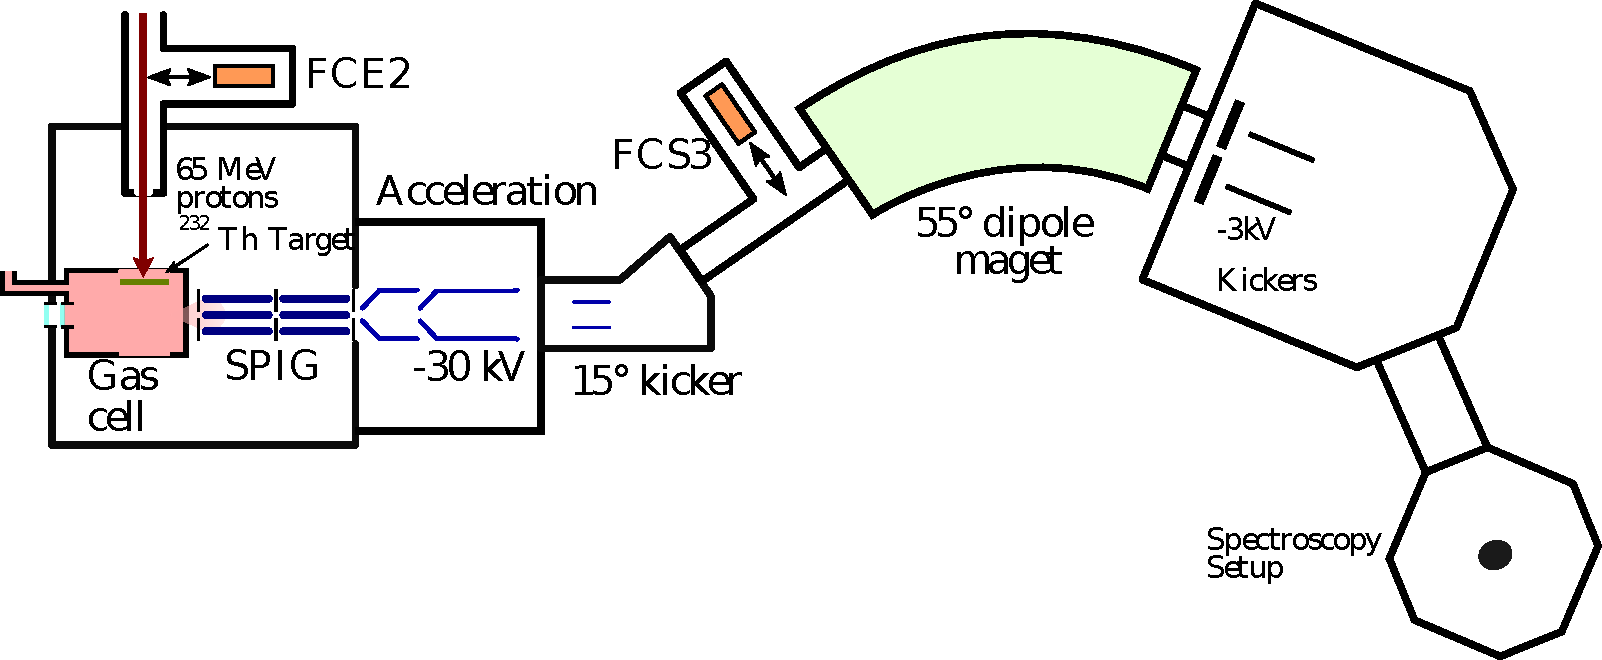
\includegraphics[width=0.8\textwidth]{IGISOL_2}\\}
		\only<3>{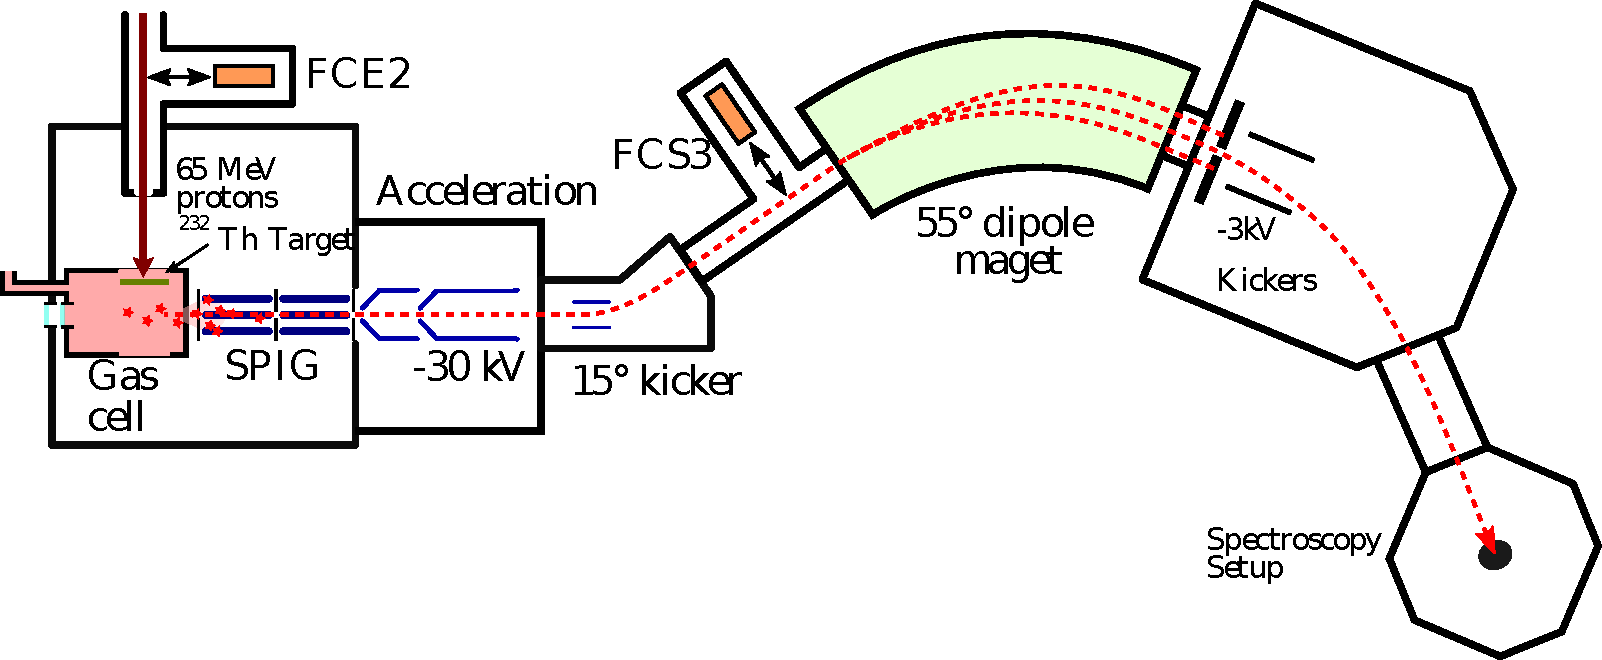
\includegraphics[width=0.8\textwidth]{IGISOL_3}\\}
	\end{overlayarea}
\end{frame}

\section{Experimental Setup}
\begin{frame}{Decay Station}
\begin{columns}
	\begin{column}{0.3\textwidth}
		\centering
		\begin{itemize}
			\item[1$\rightarrow$] BEGE2020 
			\item[3$\rightarrow$] BEGE6530 
			\item[2$\rightarrow$] QuadSi 
			\item[1$\rightarrow$] CircSi 
			\item[1$\rightarrow$] Si(Li) 
		\end{itemize}
	\end{column}
	\begin{column}{0.7\textwidth}
		\centering
		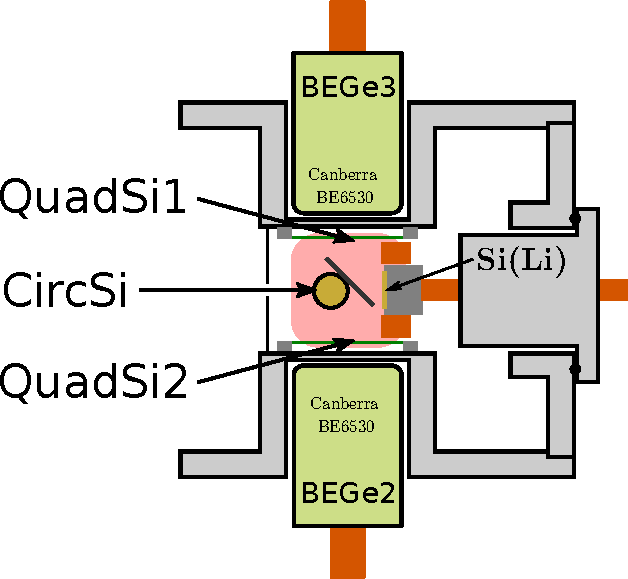
\includegraphics[width=0.9\textwidth]{top_view.pdf}\\
	\end{column}
\end{columns}
\end{frame}

\section{Efficiency Test}
\begin{frame}{Sources}
	\begin{columns}
		\begin{column}{0.5\textwidth}
			\begin{overlayarea}{\textwidth}{\textheight}
				\centering
				%\vspace{0.1\textheight}
				\color{red}{Detection Efficiency\\ of the different detectors}
				\vspace{0.1\textheight}

				\begin{itemize}
					\item[1$\rightarrow$]{3-$\alpha$ source \\
										\small$^{239}$Pu - $^{241}$Am - $^{244}$Cm}
					\item[5$\rightarrow$]{$\gamma$ sources \\
										\small $^{133}$Ba - $^{210}$Pb - $^{60}$Co \\
										$^{137}$Cs - $^{152}$Eu}
					%\item[1$\rightarrow$]{$\alpha$-recoil source\\
%										\small $^{223}$Ra}
				\end{itemize}
				\center
				\vspace{0.1\textheight}
				\hspace{-0.2\textwidth}
			\end{overlayarea}
		\end{column}
		\begin{column}{0.5\textwidth}
			\begin{overlayarea}{\textwidth}{\textheight}
				\centering
				\vspace{-0.12\textheight}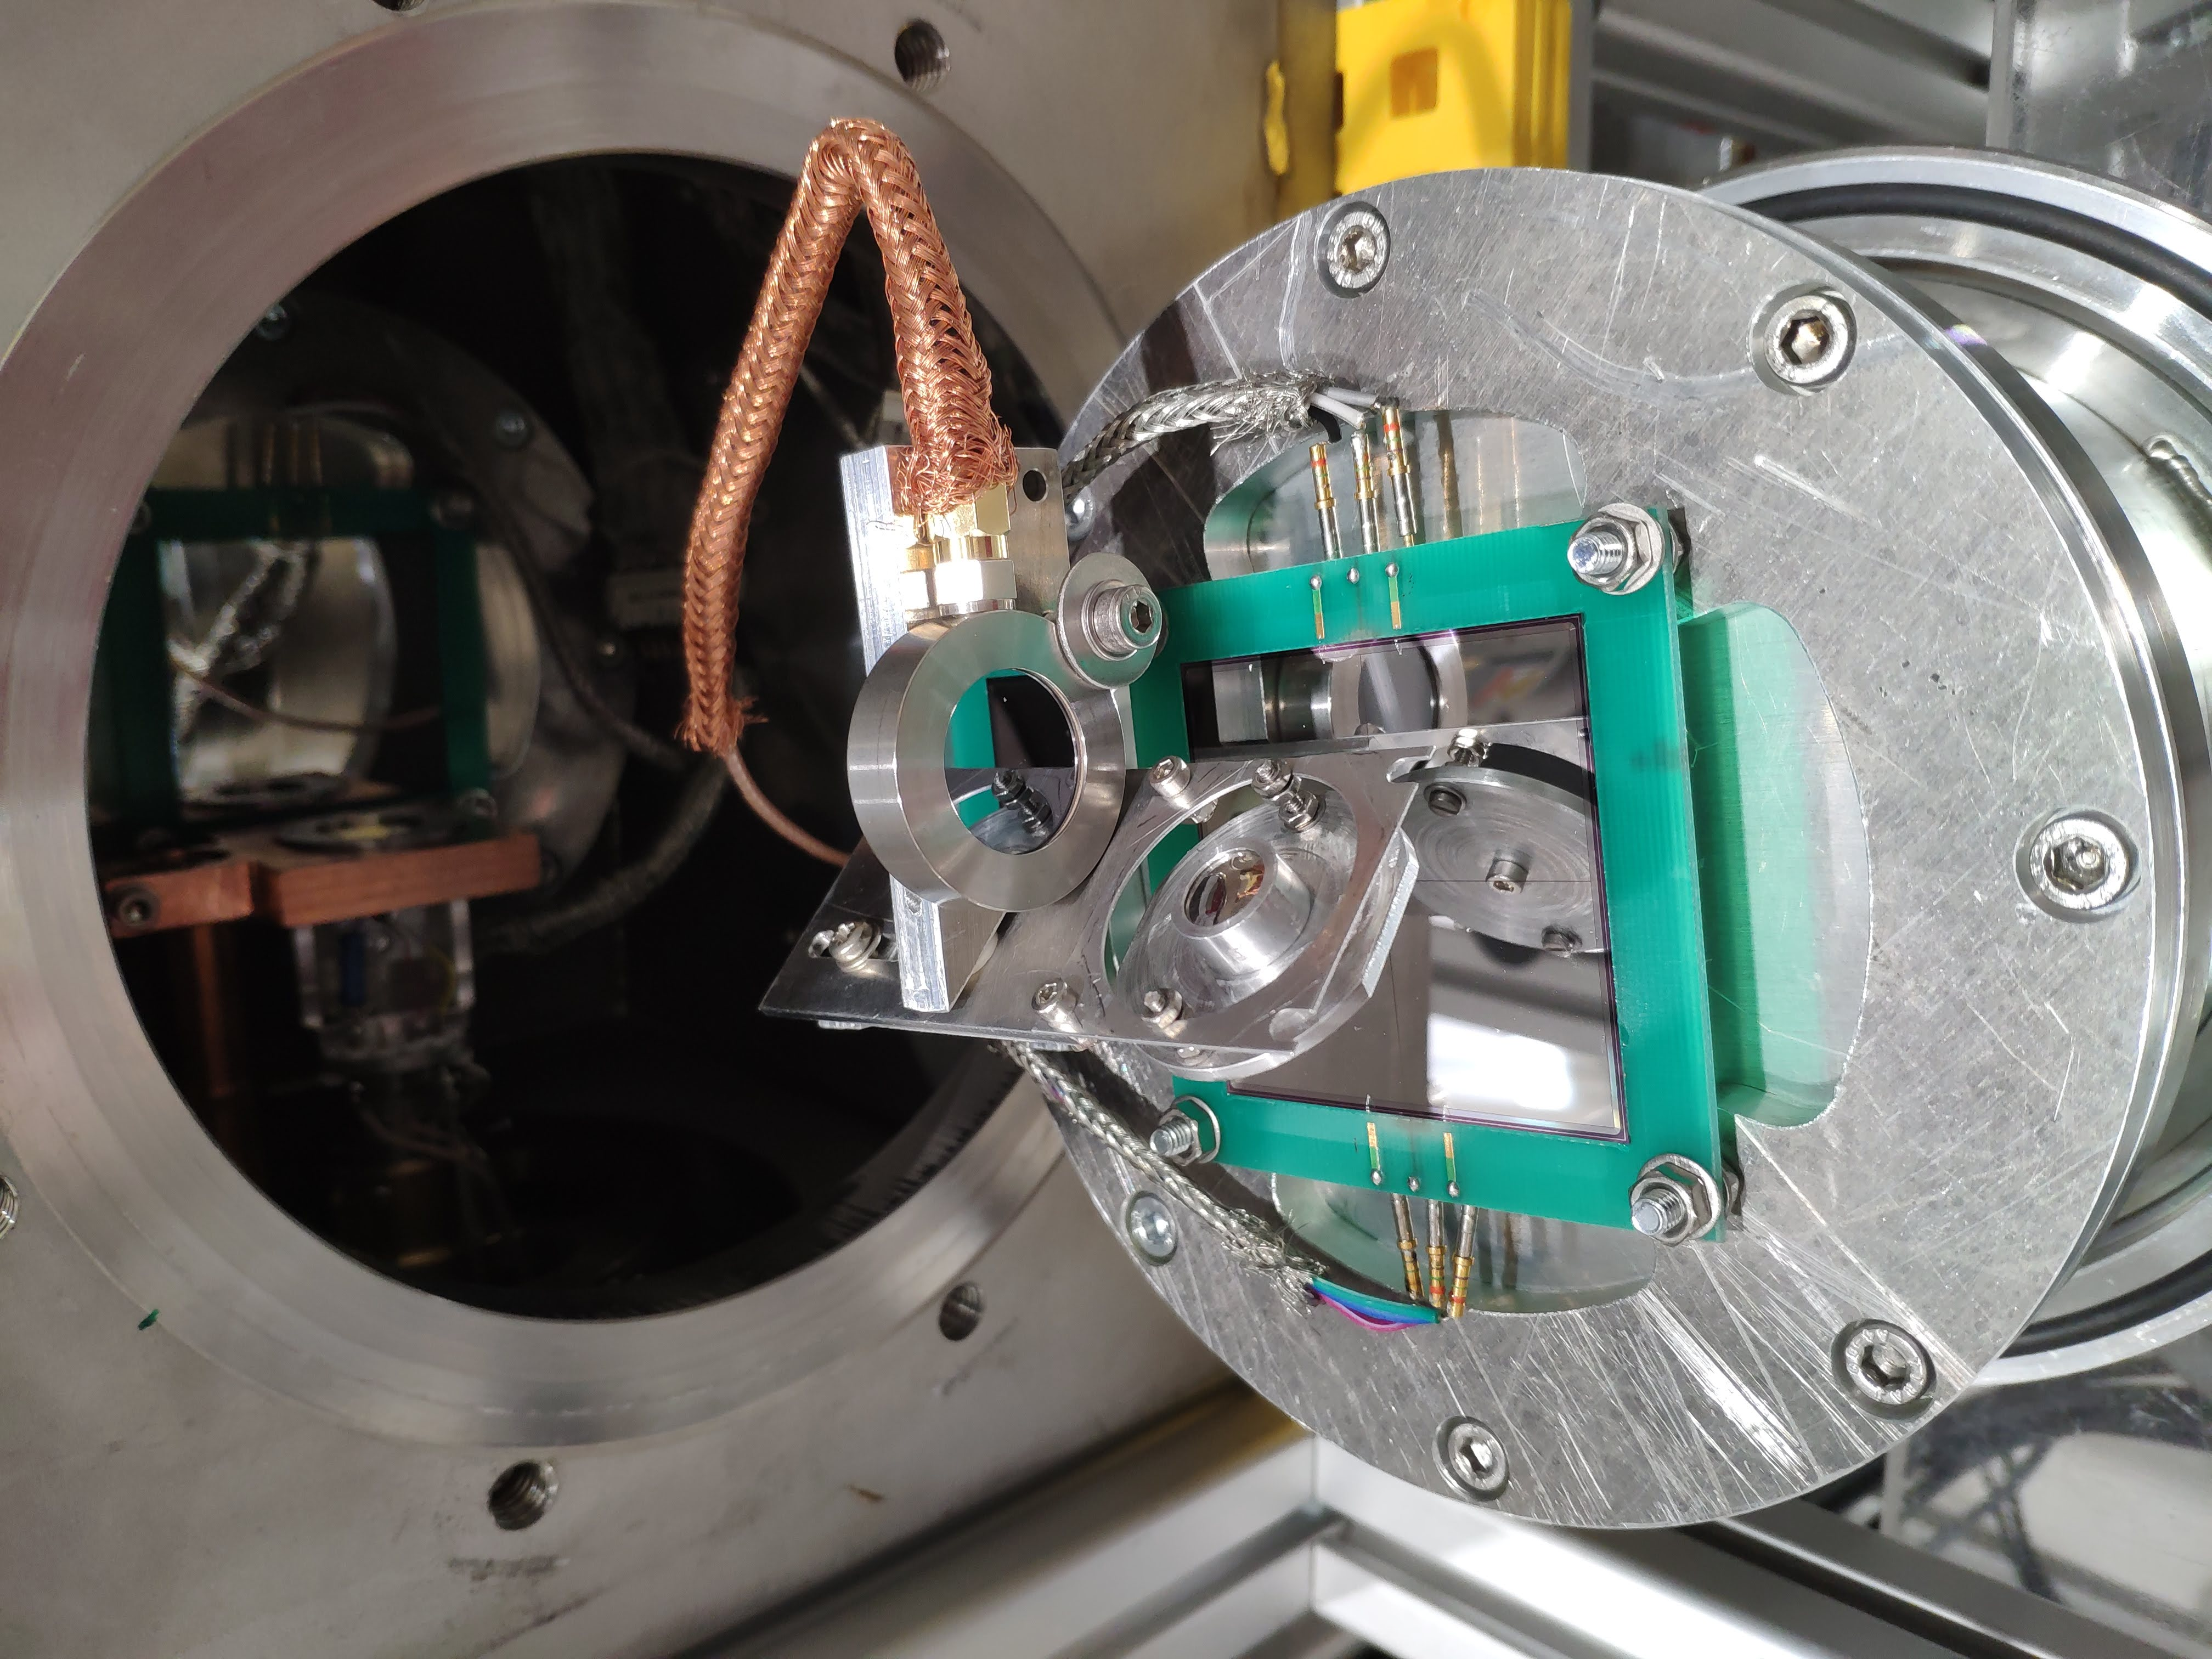
\includegraphics[angle=-90,origin=c,width=0.45\textwidth]{3alpha.jpg}
				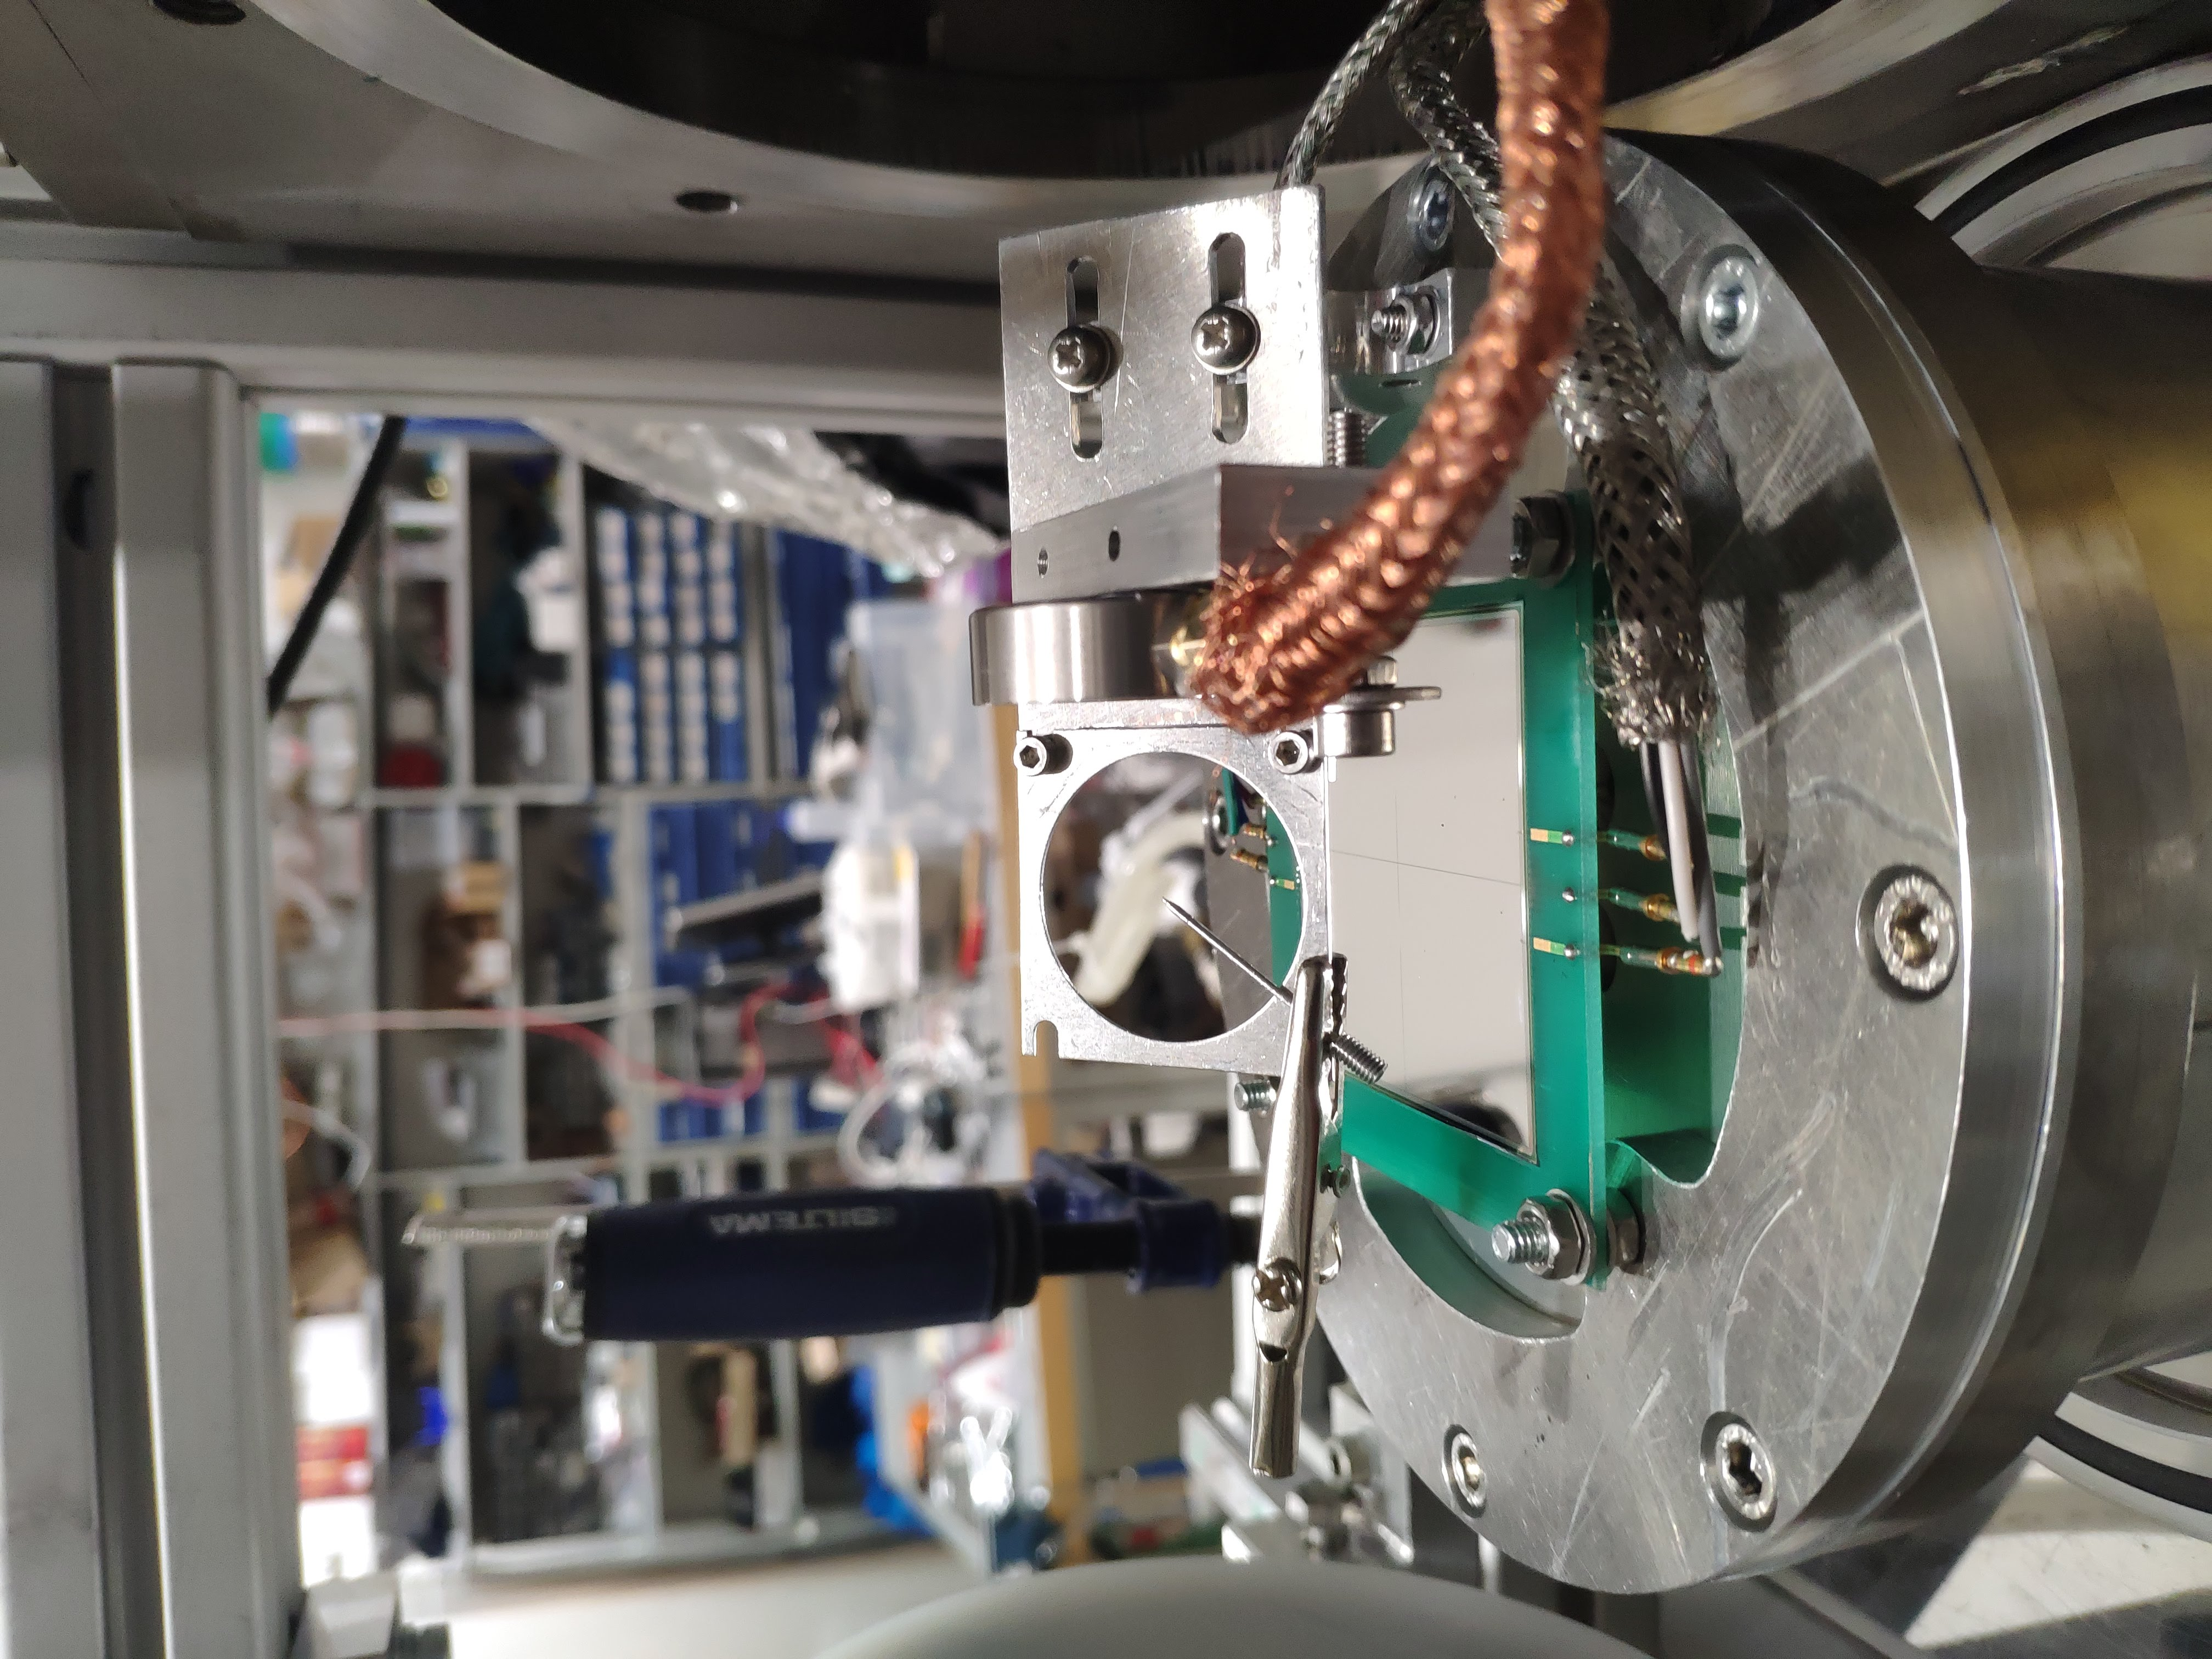
\includegraphics[angle=-90,origin=c,width=0.45\textwidth]{alpharec.jpg}\\
				\vspace{0.01\textheight}
				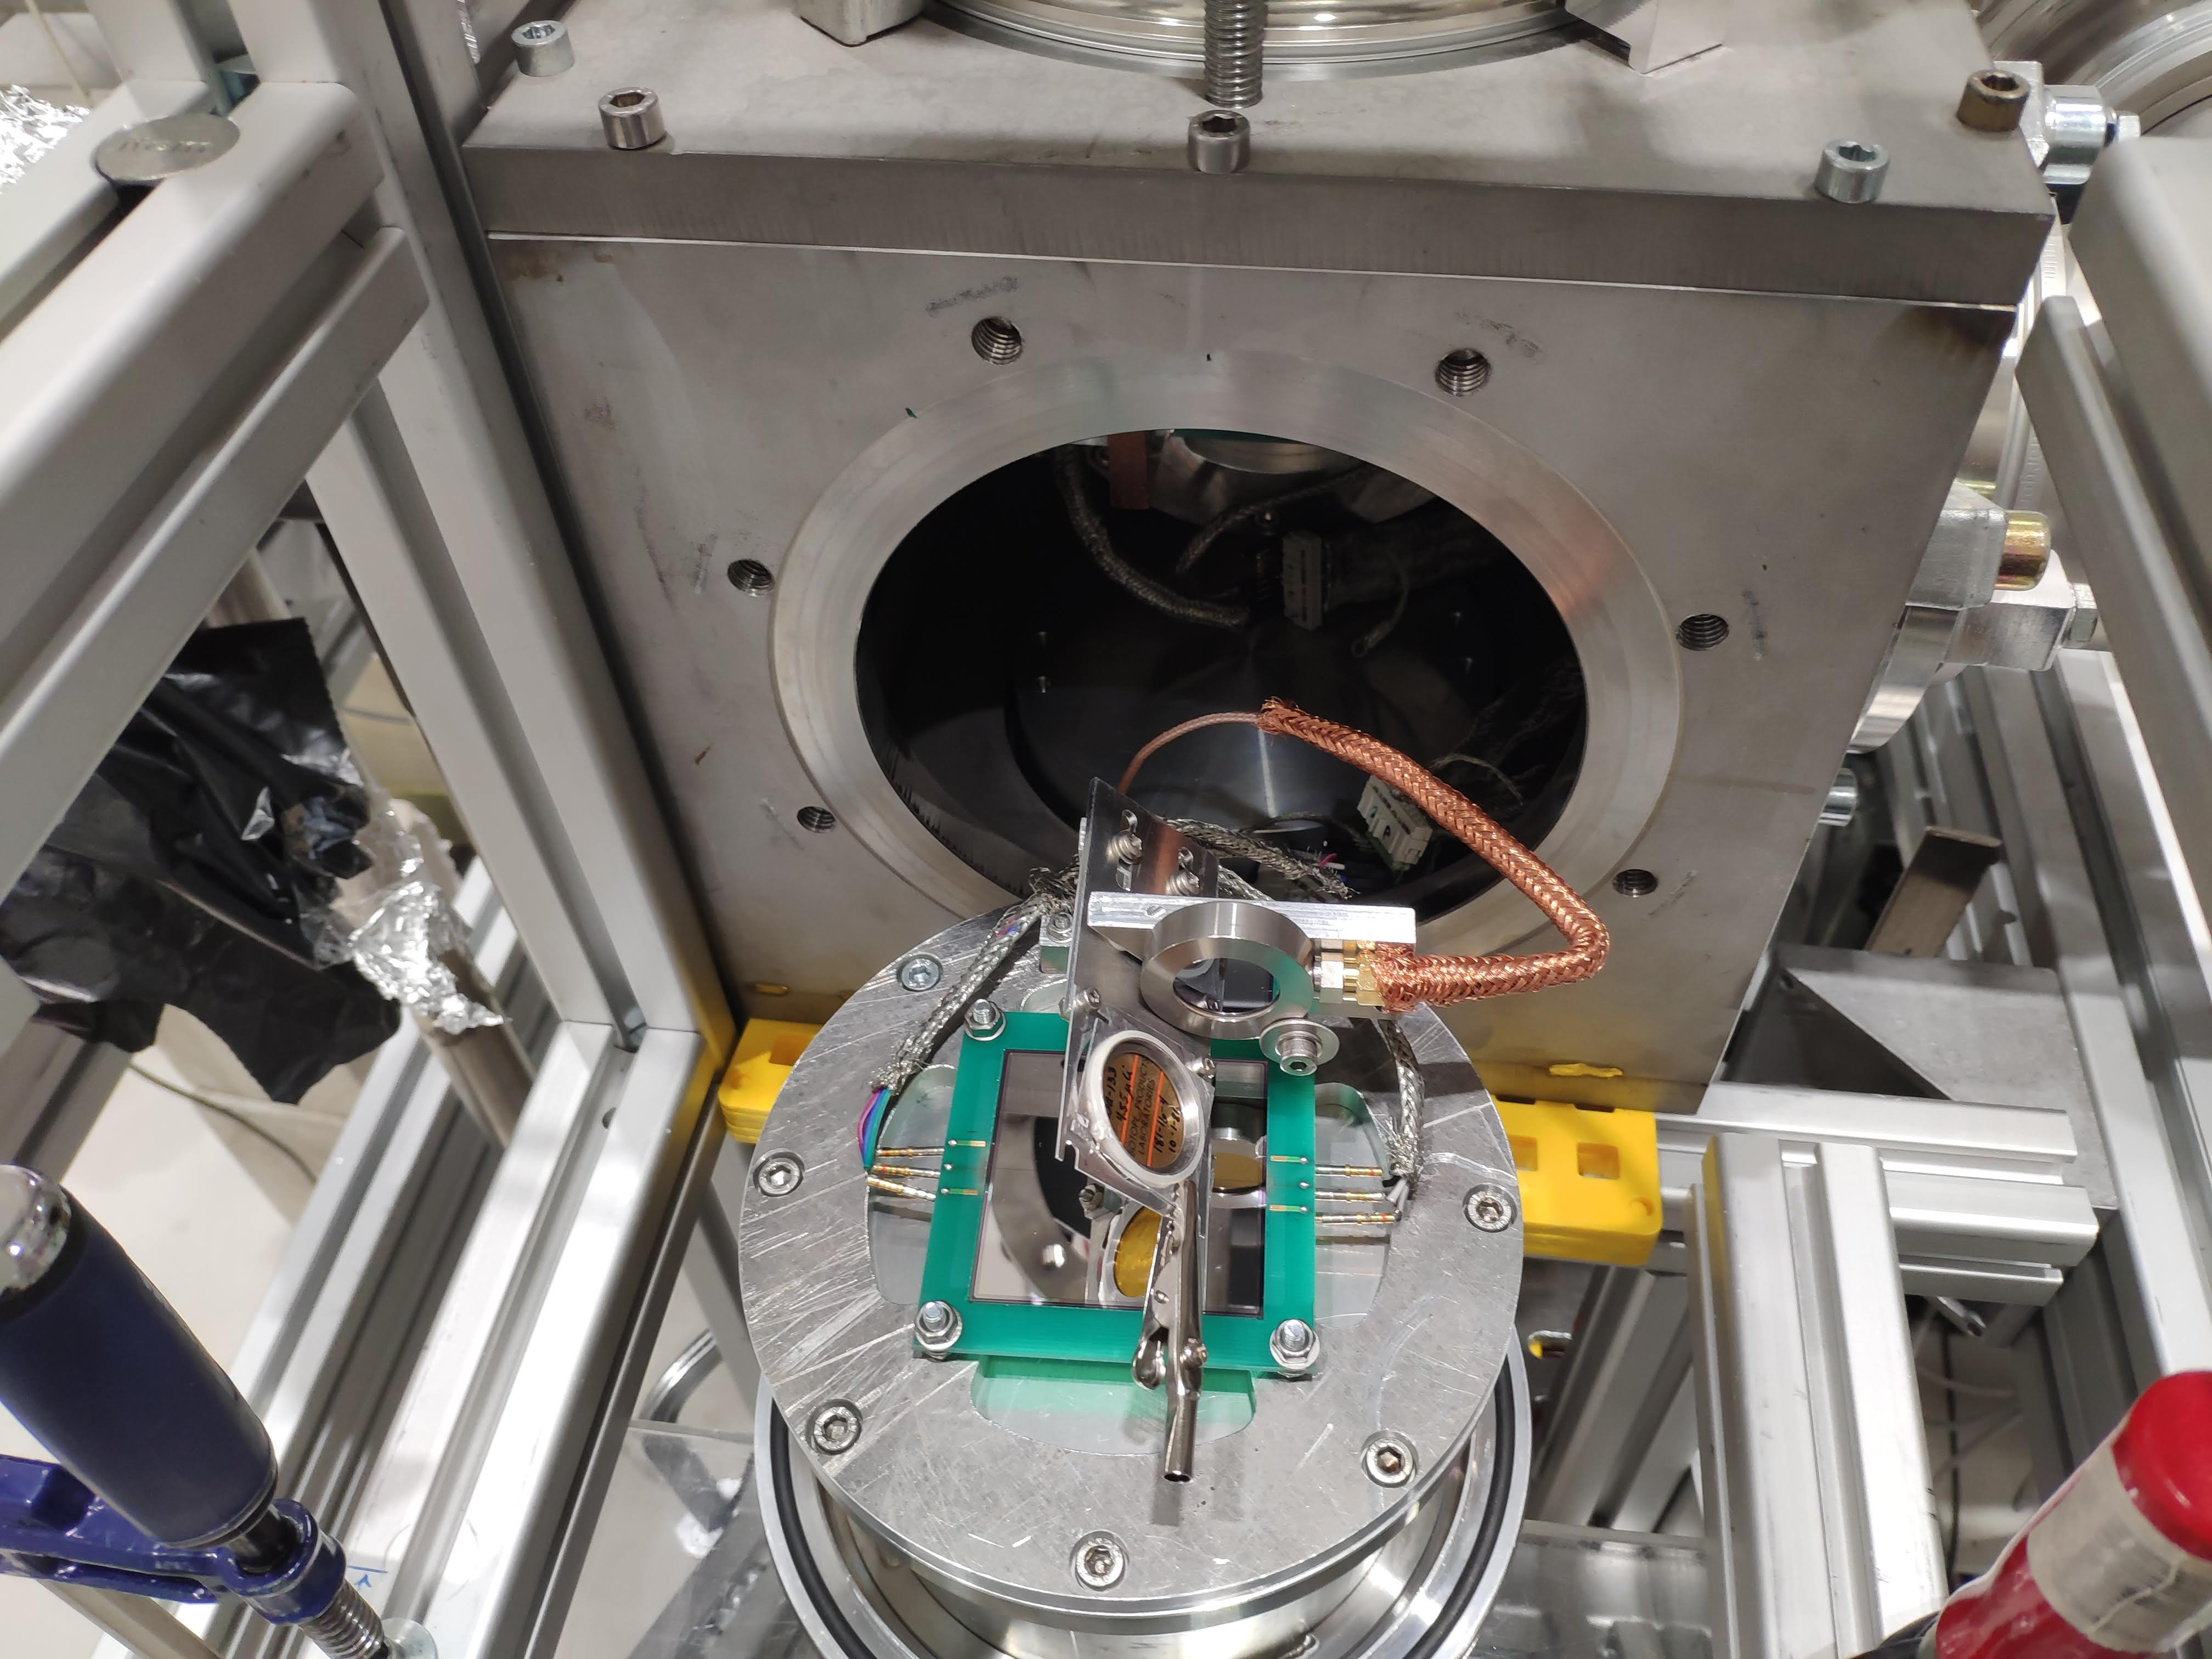
\includegraphics[width=0.925\textwidth]{gammasrc.jpg}
			\end{overlayarea}
		\end{column}
	\end{columns}
\end{frame}

\begin{frame}{Method}
	\begin{columns}
		\begin{column}{0.4\textwidth}
			\begin{overlayarea}{\textwidth}{\textheight}
				\centering
				\small
				\[ \mathcal{E}_{\text{ABS}} = \dfrac{\text{Peak Area}}{\text{Time}\times \text{Activity}\times \text{Intensity}}\]
				\begin{itemize}
					\item[$\rightarrow$] Peak Area
					\item[$\rightarrow$] Time
					\item[$\rightarrow$]	 Activity
					\item[$\rightarrow$] Intensity
				\end{itemize}
			\end{overlayarea}
		\end{column}
		\begin{column}{0.6\textwidth}
			\begin{overlayarea}{\textwidth}{\textheight}
				\centering
				\vspace{0.15\textheight}
				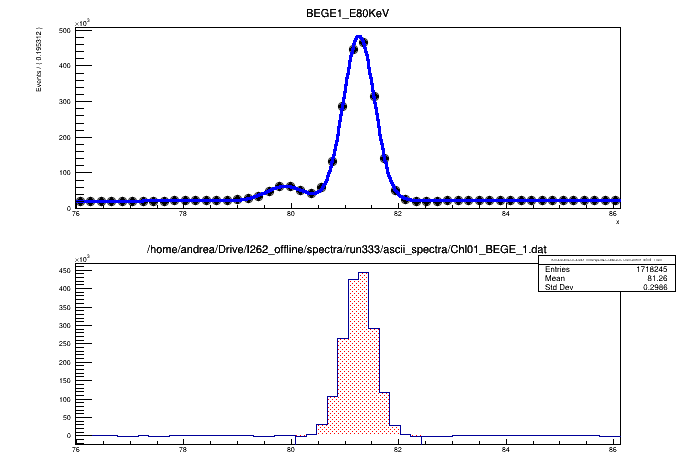
\includegraphics[width=\textwidth]{BEGE1_E80KeV.png}
			\end{overlayarea}
		\end{column}
	\end{columns}
\end{frame}

\begin{frame}{Results}
	\centering
	\vspace{-0.07\textheight}
	\textbf{BEGE detectors}\\
	\vspace{0.01\textheight}
	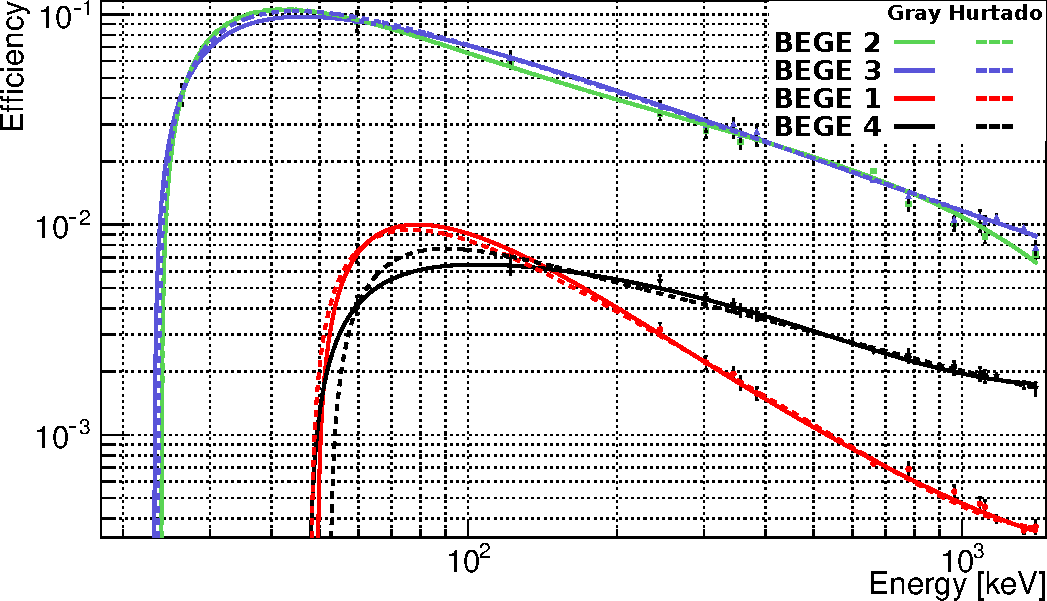
\includegraphics[width=0.7\textwidth]{BEGE_final.pdf}
	\small
	$\footnote{\tiny Hurtado Garcia-Lenon Nucl. Instr. and Meth. A 594 (2008) 362–367} \mathcal{E}_{\text{ABS}} (E) = a_1 \left(\exp \left(-a_2 E^{a_3}\right)+\exp \left(-a_4 E^{a_5}\right)	\right)\left(1-\exp \left(a_6 E^{a_7}\right)\right) $\\
	$\footnote{\tiny P.W. Gray, A. Ahmad, Nucl. Instr. and Meth. A 237 (1985) 577} \mathcal{E}_{\text{ABS}} (E) = \dfrac{1}{E}\sum_i a_i \left(\ln(E)\right)^{i-1}$
\end{frame}

\begin{frame}{Results}
	\centering
	\vspace{-0.1\textheight}
	\textbf{Silicon Detectors}\\
	\vspace{0.05\textheight}
	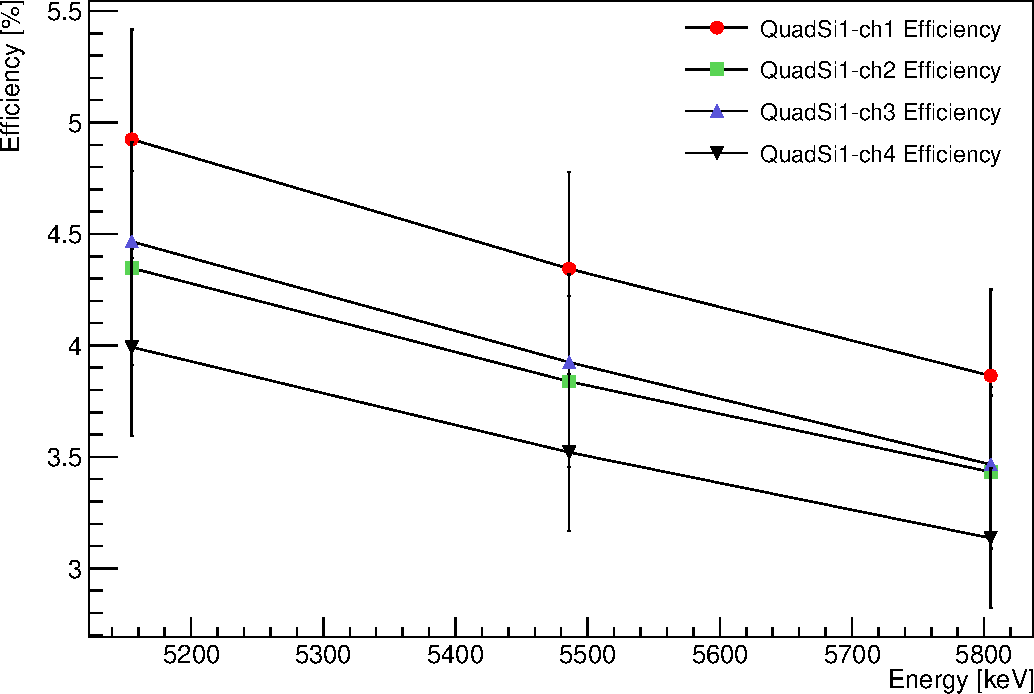
\includegraphics[width=0.45\textwidth]{QuadSi1.pdf}
	\hspace{0.05\textwidth}
	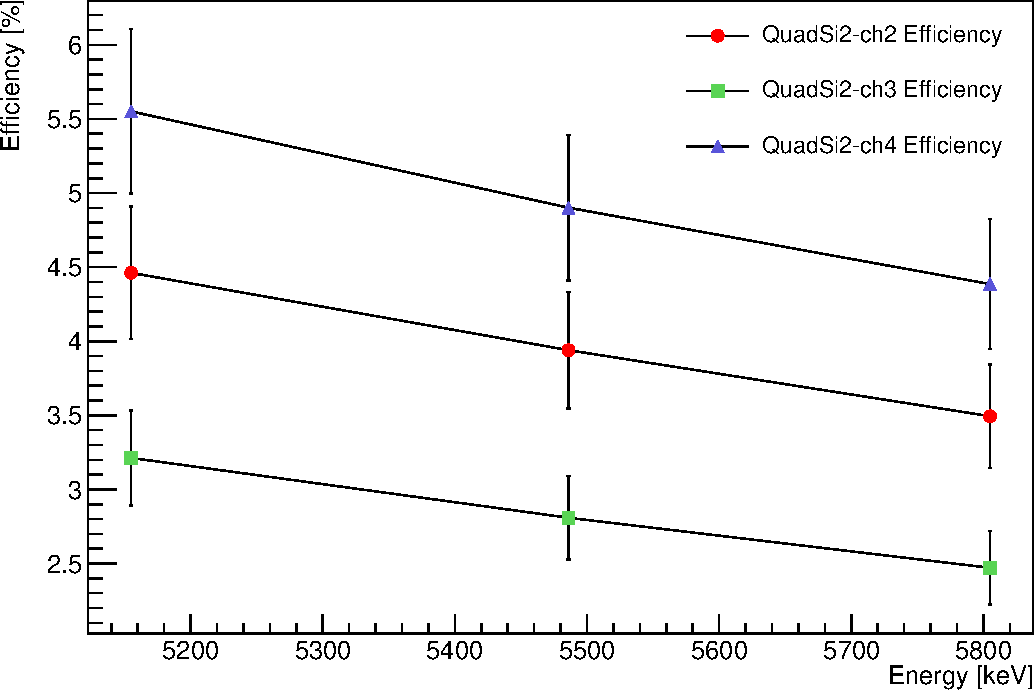
\includegraphics[width=0.45\textwidth]{QuadSi2.pdf}\\
	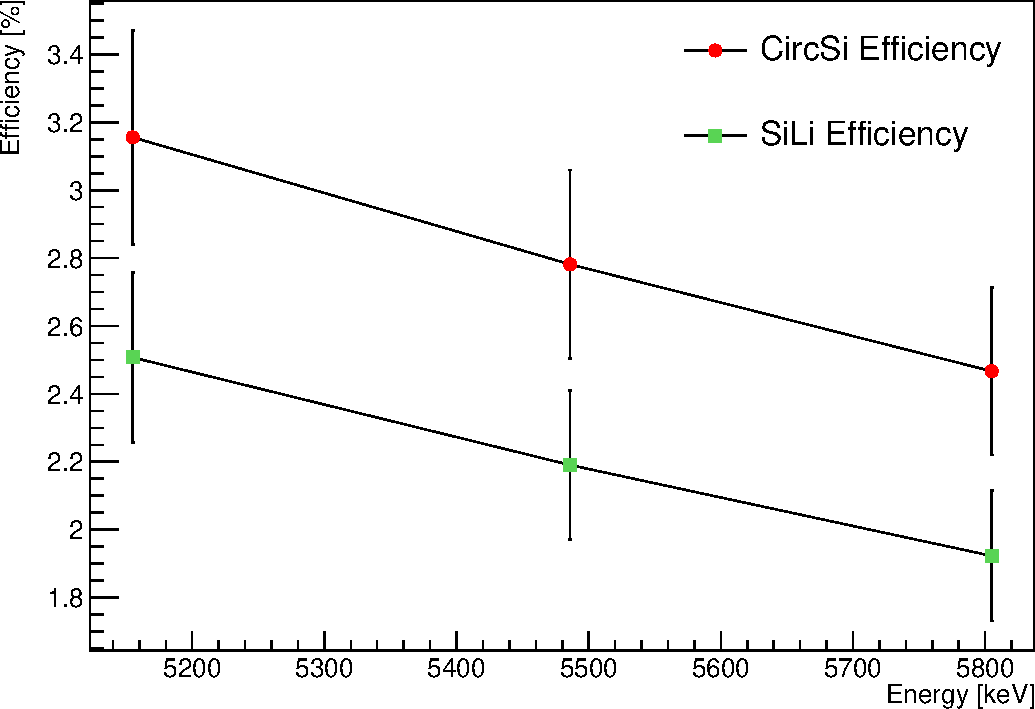
\includegraphics[width=0.45\textwidth]{SiLi_CircSi.pdf}
\end{frame}

\section{Conclusion}
\begin{frame}{Summary}
	\centering
	\begin{itemize}
		\item Efficiency in agreement with the expected values
		\item Compare Si detectors efficiency from $^{223}$Ra recoil source
		\item Start analysis of first experimental isobar at A=227
		\
	\end{itemize}
\end{frame}

% \section*{}
% \begin{frame}{}
% 	\centering
% 	\vspace{-0.01\textheight}
% 	\hspace*{-0.2\textwidth}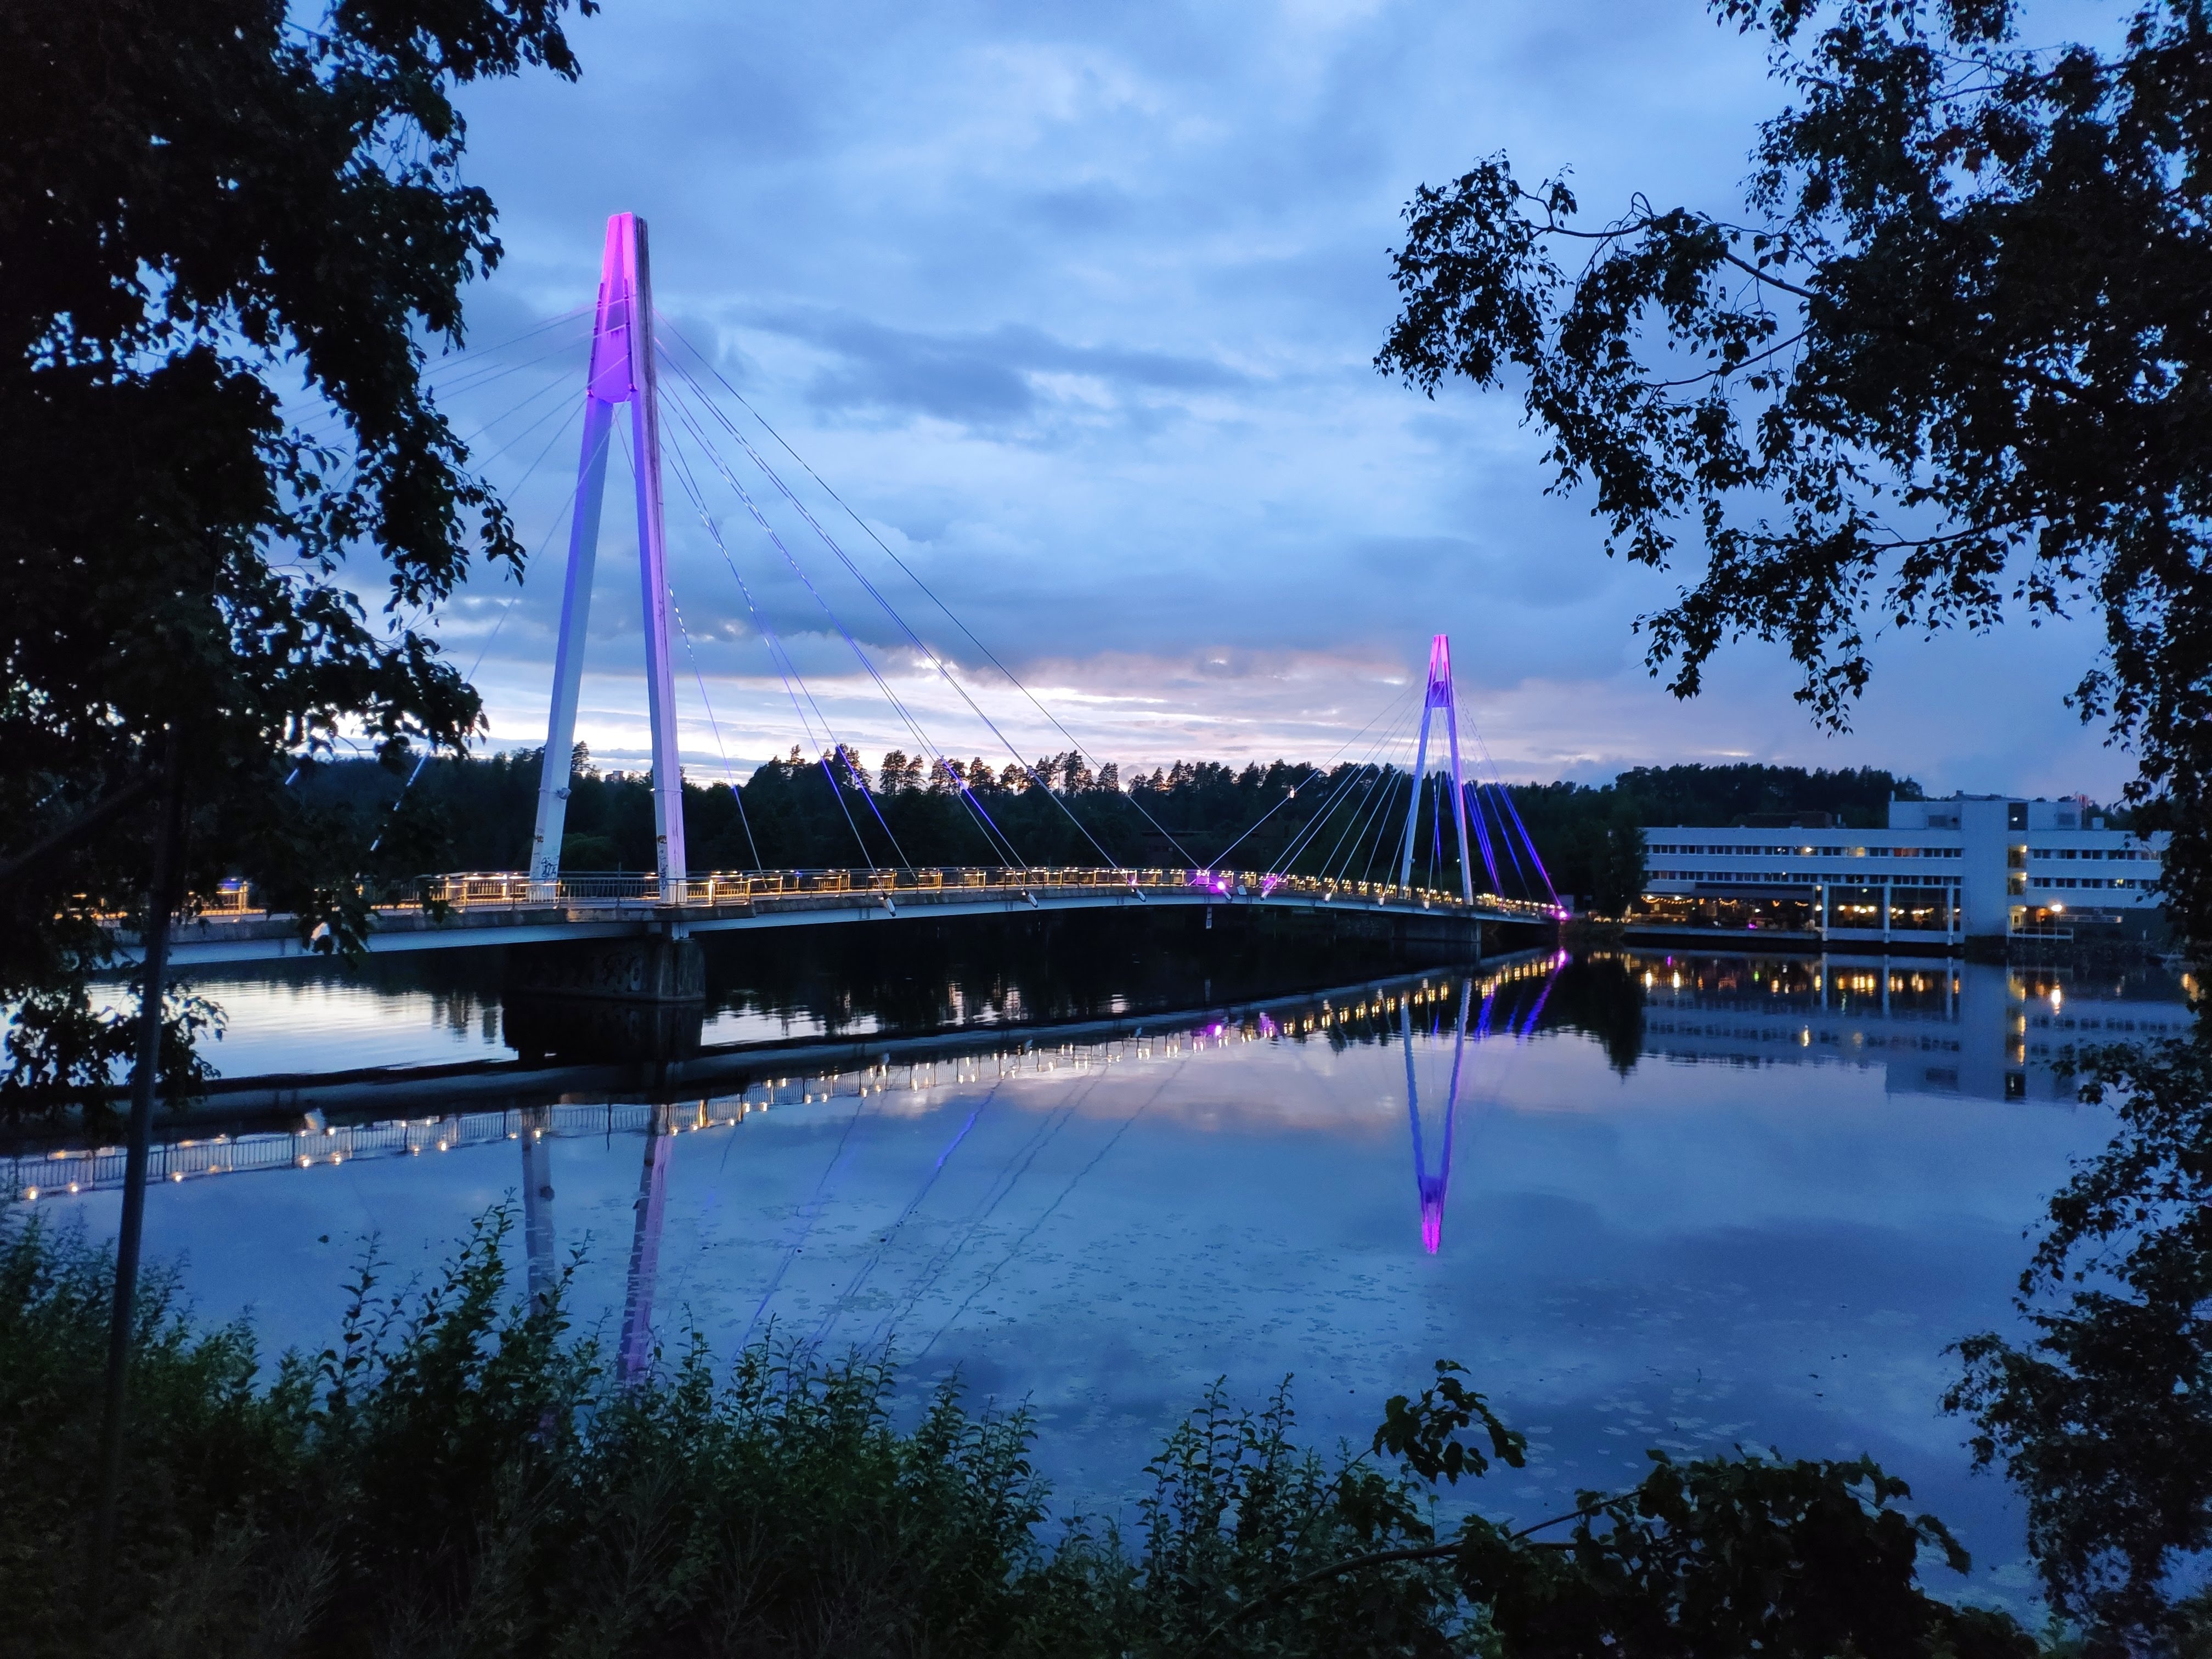
\includegraphics[width=1.3\textwidth]{bridge.jpg}\\
% \end{frame}

\end{document}

